% Copyright (c) 2015 Daniele Masini - d.masini.it@gmail.com

\chapter{Congruenza nei triangoli}\label{chap:congruenza_nei_triangoli}

\includegraphics[width=0.95\textwidth]{triangle_shapes.jpg}
  \begin{center}
    {\large ``Triangle Shapes''}\par
    Foto di maxtodorov\par
    \url{http://www.flickr.com/photos/maxtodorov/3066505212/}\par
    Licenza: Creative Commons Attribution\par
  \end{center}
\newpage

\section{Definizioni relative ai triangoli}\label{sect:definizioni_triangoli}

Definiamo gli elementi principali di un triangolo
\begin{definizione}~
\begin{itemize*}
\item Un \emph{triangolo} è un poligono di tre lati.
\item Si chiamano \emph{vertici} gli estremi dei lati.
\item Un vertice si dice \emph{opposto a un lato} se non appartiene a quel lato.
\item Si chiamano \emph{angoli interni} del triangolo i tre angoli formati dai lati.
\item Un angolo interno si dice \emph{angolo compreso tra due lati} quando i lati dell'angolo contengono dei lati del triangolo.
\item Un angolo interno si dice \emph{angolo adiacente a un lato} del triangolo quando uno dei suoi lati contiene quel lato del triangolo.
\item Un angolo si dice \emph{angolo esterno} al triangolo se è un angolo adiacente a un angolo interno.
\item Si dice \emph{bisettrice} relativa a un vertice, il segmento di bisettrice dell'angolo al vertice che ha per estremi il vertice stesso e il punto in cui essa incontra il lato opposto.
\item Si dice \emph{mediana} relativa a un lato il segmento che ha per estremi il punto medio del lato e il vertice opposto a quel lato.
\item Si dice \emph{altezza} di un triangolo relativa a un suo lato il segmento di perpendicolare che ha per estremi il vertice opposto al lato e il punto di intersezione della perpendicolare con la retta contenente il lato. 
\item Si dice \emph{asse} di un triangolo, relativo a un suo lato, la perpendicolare al lato condotta nel suo punto medio.
\end{itemize*}
\end{definizione}

Nel triangolo (a) della figura seguente, $A$, $B$ e $C$ sono i vertici del triangolo, il vertice $A$ è opposto al lato $a$, l'angolo $\alpha$ è interno al triangolo ed è compreso tra i lati $AB$ e $AC$, mentre l'angolo $\beta$ è esterno. Nel triangolo (b) $AL$ è la bisettrice dell'angolo nel vertice $A$, $AH$ è altezza relativa alla base $BC$, $AM$ è la mediana relativa al lato $BC$ e la retta $r$ è l'asse di $BC$.

\begin{figure}[htb]
\centering% Copyright (c) 2015 Daniele Masini - d.masini.it@gmail.com

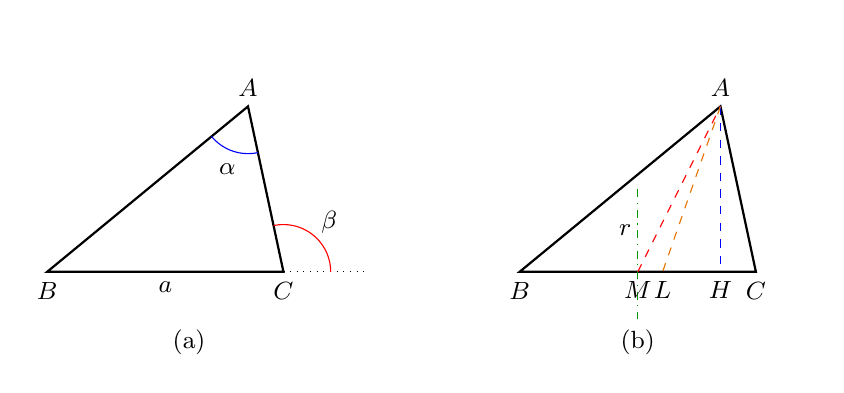
\begin{tikzpicture}[scale=1.5,font=\small]
\usetikzlibrary{calc}

\begin{scope}

\coordinate (b) at (0,0);
\coordinate (a) at (1.7,1.4);
\coordinate (c) at (2,0);

\draw[thick] (b) node[below] {$B$} -- node[below,midway] {$a$} (c) node[below] {$C$} -- (a) node[above] {$A$} -- cycle;
\draw[dotted] (c) -- ($(b)!1.35!(c)$) coordinate (d);

\begin{scope}
\clip (c) -- (d) -- (2.5,1) -- (a) -- cycle;
\draw[red] (c) circle (0.4);
\end{scope}
\node at ([shift={(11pt,12pt)}]c) {$\beta$};

\begin{scope}
\clip (b) -- (a) -- (c) -- cycle;
\draw[blue] (a) circle (0.4);
\end{scope}
\node at ([shift={(-5pt,-15pt)}]a) {$\alpha$};

\node at (1.2,-0.6) {(a)};

%\node at (2.5,1.2) {angolo};
%\node at (2.5,0.9) {esterno};
\end{scope}

\begin{scope}[xshift=4cm]

\coordinate (b) at (0,0);
\coordinate (a) at (1.7,1.4);
\coordinate (c) at (2,0);

\draw[thick] (b) node[below] {$B$} -- (c) node[below] {$C$} -- (a) node[above] {$A$} -- cycle;

%\begin{scope}
%\clip (b) -- (a) -- (c) -- cycle;
%\draw (a) node[left=3pt, below=15pt] {$\alpha$} circle (0.4);
%\end{scope}

\coordinate (m) at ($(b)!0.5!(c)$);

\draw[green!60!black,dashdotted] ($(m)!0.7cm!90:(c)$) coordinate (r) -- ($(m)!-.4cm!90:(c)$); % asse
\node at ([shift={(-3pt,-10pt)}]r) {$r$};
\draw[red,dashed] (m) node[black,below] {$M$} -- (a); % mediana
\draw[blue,dashed] (a) -- ($(b)!(a)!(c)$) node[black,below] {$H$}; % altezza

\node [circle] (circ1) at (a) [minimum size=2cm] {}; % circonferenza con centro in A
\coordinate (u) at (intersection of a--b and circ1);
\coordinate (v) at (intersection of a--c and circ1);
\node [circle] (circ2) at (u) [minimum size=2cm] {}; % circonferenza con centro in U
\node [circle] (circ3) at (v) [minimum size=2cm] {}; % circonferenza con centro in V
\coordinate (bis) at (intersection 1 of circ2 and circ3);
% la bisettrice di A passa per A e per bis1
\coordinate (bi) at ($(a)!5!(bis)$);
\coordinate (bt) at (intersection of b--c and a--bi);
\draw[orange!90!black,dashed] (a) -- (bt) node [black,below] {$L$}; % bisettrice


\node at (1,-0.6) {(b)};
\end{scope}

\end{tikzpicture}

%\caption{Triangolo. Vertici, angoli, bisettrice, mediana, asse.}\label{fig:triangolo1}
\end{figure}

I triangoli possono essere classificati rispetto ai lati
\begin{definizione}~
\begin{itemize*}
\item un triangolo si dice \emph{equilatero} se ha i tre lati congruenti;
\item un triangolo si dice \emph{isoscele} se ha (almeno) due lati congruenti;
\item un triangolo si dice \emph{scaleno} se ha i lati a due a due non congruenti.
\end{itemize*}
\end{definizione}

\begin{figure}[htb]
\centering% Copyright (c) 2015 Daniele Masini - d.masini.it@gmail.com

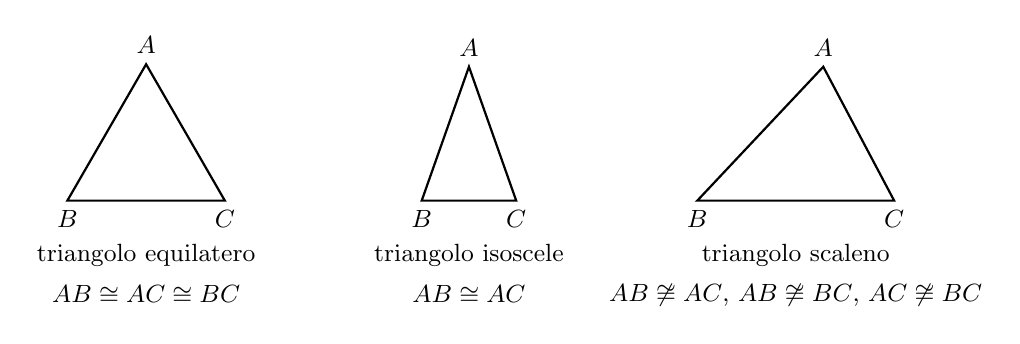
\begin{tikzpicture}[scale=1,font=\small]
\usetikzlibrary{calc}

\begin{scope}
\coordinate (b) at (0,0);
\coordinate (c) at (2,0);

\draw[thick] (b) node[below] {$B$} -- (c) node[below] {$C$} -- +(120:2) coordinate (a) node[above] {$A$} -- cycle;

\node at (1,-0.7) {triangolo equilatero};
\node at (1,-1.2) {$AB\cong AC\cong BC$};
\end{scope}

\begin{scope}[xshift=4.5cm]
\coordinate (b) at (0,0);
\coordinate (a) at (0.6,1.7);
\coordinate (c) at (1.2,0);

\draw[thick] (b) node[below] {$B$} -- (c) node[below] {$C$} -- (a) node[above] {$A$} -- cycle;

\node at (.6,-0.7) {triangolo isoscele};
\node at (.6,-1.2) {$AB\cong AC$};
\end{scope}


\begin{scope}[xshift=8cm]
\coordinate (b) at (0,0);
\coordinate (a) at (1.6,1.7);
\coordinate (c) at (2.5,0);

\draw[thick] (b) node[below] {$B$} -- (c) node[below] {$C$} -- (a) node[above] {$A$} -- cycle;

\node at (1.25,-0.7) {triangolo scaleno};
\node at (1.25,-1.2) {$AB\not\cong AC$, $AB\not\cong BC$, $AC\not\cong BC$};
\end{scope}

\end{tikzpicture}

\caption{Classificazione di un triangolo rispetto ai lati}\label{fig:class_triangolo_lati}
\end{figure}

\noindent o rispetto agli angoli
\begin{definizione}~
\begin{itemize*}
\item un triangolo si dice \emph{rettangolo} se ha un angolo interno retto; in un triangolo rettangolo si chiama \emph{ipotenusa} il lato che si oppone all'angolo retto e si chiamano \emph{cateti} i lati adiacenti all'angolo retto;
\item un triangolo si dice \emph{ottusangolo} se ha un angolo interno ottuso;
\item un triangolo si dice \emph{acutangolo} se ha tutti gli angoli interni acuti.
\end{itemize*}
\end{definizione}

\begin{figure}[htb]
\centering% Copyright (c) 2015 Daniele Masini - d.masini.it@gmail.com

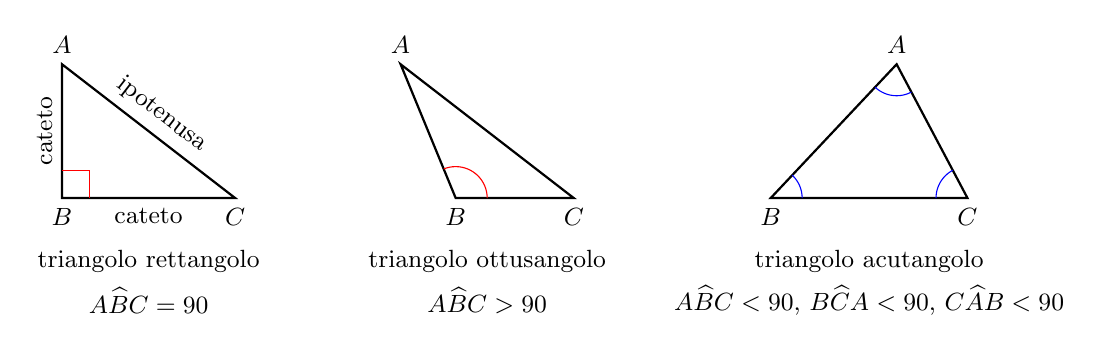
\begin{tikzpicture}[scale=1,font=\small]
\usetikzlibrary{calc}

\begin{scope}
\coordinate (a) at (0,1.7);
\coordinate (b) at (0,0);
\coordinate (c) at (2.2,0);

\draw[thick] (b) node[below] {$B$} -- node[below,midway,sloped] {cateto} (c) node[below] {$C$} -- node[above,midway,sloped] {ipotenusa} (a) node[above] {$A$} -- cycle;
\path (b) -- node[above,midway,sloped] {cateto} (a);
\draw[red] ([shift={(10pt,0)}]b) -- ([shift={(10pt,10pt)}]b) -- ([shift={(0pt,10pt)}]b);

\node at (1.1,-0.8) {triangolo rettangolo};
\node at (1.1,-1.3) {$A\widehat{B}C=90\grado$};
\end{scope}

\begin{scope}[xshift=5cm]
\coordinate (b) at (0,0);
\coordinate (a) at (-0.7,1.7);
\coordinate (c) at (1.5,0);

\draw[thick] (b) node[below] {$B$} -- (c) node[below] {$C$} -- (a) node[above] {$A$} -- cycle;

\begin{scope}
\clip (a) -- (b) -- (c) -- (1.5,1.7) -- cycle;
\draw[red] (b) circle (0.4);
\end{scope}

\node at (.4,-0.8) {triangolo ottusangolo};
\node at (.4,-1.3) {$A\widehat{B}C>90\grado$};
\end{scope}

\begin{scope}[xshift=9cm]
\coordinate (b) at (0,0);
\coordinate (a) at (1.6,1.7);
\coordinate (c) at (2.5,0);

\draw[thick] (b) node[below] {$B$} -- (c) node[below] {$C$} -- (a) node[above] {$A$} -- cycle;

\begin{scope}
\clip (a) -- (b) -- (c) -- cycle;
\draw[blue] (b) circle (0.4);
\draw[blue] (a) circle (0.4);
\draw[blue] (c) circle (0.4);
\end{scope}

\node at (1.25,-0.8) {triangolo acutangolo};
\node at (1.25,-1.3) {$A\widehat{B}C<90\grado$, $B\widehat{C}A<90\grado$, $C\widehat{A}B<90\grado$};
\end{scope}

\end{tikzpicture}

\caption{Classificazione di un triangolo rispetto agli angoli}\label{fig:class_triangolo_angoli}
\end{figure}

\section{Primo e secondo criterio di congruenza dei triangoli}\label{sect:primo_secondo_criterio_di_congruenza_triangoli}

Ricordiamo che due figure piane si dicono \emph{congruenti} se sono sovrapponibili, cioè se è possibile spostare una sull'altra, senza deformarle, in modo che coincidano perfettamente. 

In particolare, due triangoli sono sovrapponibili se hanno ``ordinatamente'' congruenti i tre lati e i tre angoli. Con il termine ordinatamente intendiamo che, a partire da una coppia di vertici (il primo di un triangolo ed il secondo dell'altro) procedendo lungo il contorno in senso orario, oppure antiorario, incontriamo lati tra loro congruenti e vertici di angoli tra loro congruenti. Nel caso dei triangoli, questo succede esattamente quando angoli congruenti nei due triangoli sono compresi tra coppie di lati congruenti o, in maniera equivalente, quando sono opposti a lati congruenti.

I criteri di congruenza dei triangoli ci dicono che è sufficiente conoscere la congruenza di solo alcuni elementi dei due triangoli, generalmente tre elementi di un triangolo congruenti a tre elementi dell'altro triangolo, per poter affermare che i due triangoli sono tra loro congruenti, e quindi dedurne la congruenza degli altri elementi.

Un modo tradizionale di presentare l'argomento, dovuto allo stesso Euclide, è quello di ``dimostrare'' i primi due criteri di congruenza dei triangoli facendo uso della definizione stessa di congruenza come ``uguaglianza per sovrapposizione'', e di utilizzarli successivamente per la verifica di altre proprietà.

Secondo il matematico tedesco Hilbert, il primo criterio di congruenza è invece un assioma e il secondo criterio può essere dimostrato per assurdo attraverso il primo. 

Presenteremo questi argomenti basilari alla maniera di Euclide.

\begin{teorema}[1\textsuperscript{o} Criterio di congruenza dei triangoli]
Due triangoli sono congruenti se hanno congruenti due lati e l'angolo tra essi compreso.
\end{teorema}

% figura ()
\begin{figure}[htb]
\centering% Copyright (c) 2015 Daniele Masini - d.masini.it@gmail.com

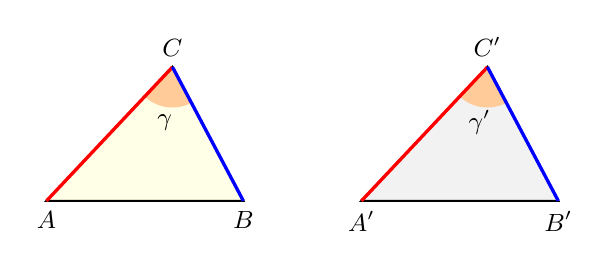
\begin{tikzpicture}[scale=1,font=\small]
\usetikzlibrary{calc}

\begin{scope}
\coordinate (a) at (0,0);
\coordinate (c) at (1.6,1.7);
\coordinate (b) at (2.5,0);
\draw[fill=yellow!10] (a) -- (b) -- (c) -- cycle;

\begin{scope}
\clip (a) -- (b) -- (c) -- cycle;
\draw[thick,orange!40,fill] (c) circle (0.5);
\node at ([shift={(-0.1,-0.7)}]c) {$\gamma$};
\end{scope}

\draw[thick] (a) node[below] {$A$} -- (b) node[below] {$B$} -- (c) node[above] {$C$} -- cycle;
\draw[red,very thick] (a) -- (c);
\draw[blue,very thick] (b) -- (c);

\end{scope}

\begin{scope}[xshift=4cm]
\coordinate (a) at (0,0);
\coordinate (c) at (1.6,1.7);
\coordinate (b) at (2.5,0);
\draw[fill=gray!10] (a) -- (b) -- (c) -- cycle;

\begin{scope}
\clip (a) -- (b) -- (c) -- cycle;
\draw[thick,orange!40,fill] (c) circle (0.5);\node at ([shift={(-0.1,-0.7)}]c) {$\gamma'$};
\end{scope}

\draw[thick] (a) node[below] {$A'$} -- (b) node[below] {$B'$} -- (c) node[above] {$C'$} -- cycle;
\draw[red,very thick] (a) -- (c);
\draw[blue,very thick] (b) -- (c);

\end{scope}

\end{tikzpicture}

\end{figure}

\noindent Ipotesi: $AC\cong A'C'$, $BC\cong B'C'$, $\gamma \cong \gamma'$.\tab Tesi:  $ABC \cong A'B'C'$.

\begin{proof}
Vogliamo dimostrare che il triangolo $A’B’C’$ può essere portato a sovrapporsi perfettamente al triangolo $ABC$.
A tal proposito, portiamo il punto $C’$ sul punto $C$ in modo tale che la semiretta $C’A’$ sia sovrapposta alla semiretta $CA$ ed i punti $B$ e $B’$ siano nello stesso semipiano individuato dalla retta $AC$.
%Dopo questo movimento, i triangoli potrebbero trovarsi nella posizione della figura a lato?
Poiché per ipotesi i segmenti $AC$ e $A’C’$ sono congruenti, se $C$ coincide con $C’$ anche $A$ deve coincidere con $A’$.
%, mentre nella figura $A’C’$ è maggiore di $AC$. Né $A'$ può cadere all'interno di $AC$. In definitiva $C\equiv C'$ e $A\equiv A'$.

%Allora i triangoli potrebbero trovarsi almeno nella seguente posizione, nella quale $A$ e $A’$ coincidono?
%Tuttavia nemmeno questa posizione è possibile poiché
Avendo supposto per ipotesi che gli angoli $\gamma$ e $\gamma’$ sono congruenti, la semiretta per $CB$ e la semiretta per $C’B’$ devono sovrapporsi, in quanto devono formare lo stesso angolo con la semiretta per $CA$, ovvero per $C'A'$.

%A questo punto, rimane da fissare la posizione di $B’$ rispetto a $B$, cioè rimane da decidere se $B’$ cade internamente al segmento $CB$, come nella figura che segue, se $B’$ cade esternamente al segmento $CB$ o se $B’$ e $B$ coincidono.
Inoltre, poiché per ipotesi $BC\cong B'C'$, il punto $B’$ deve necessariamente coincidere con $B$.

Pertanto tutti i vertici del triangolo $A'B'C'$ si sovrappongono ai vertici del triangolo $ABC$ e di conseguenza i triangoli $ABC$ e $A’B’C’$ sono congruenti.
\end{proof}

\begin{teorema}[2\textsuperscript{o} Criterio di congruenza dei triangoli]
Due triangoli sono congruenti se hanno congruenti due angoli e il lato tra essi compreso.
\end{teorema}

\begin{figure}[htb]
\centering% Copyright (c) 2015 Daniele Masini - d.masini.it@gmail.com

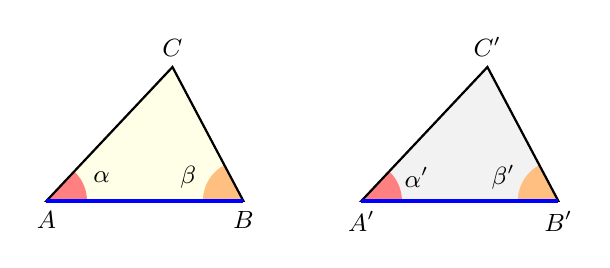
\begin{tikzpicture}[scale=1,font=\small]
\usetikzlibrary{calc}

\begin{scope}
\coordinate (a) at (0,0);
\coordinate (c) at (1.6,1.7);
\coordinate (b) at (2.5,0);
\draw[fill=yellow!10] (a) -- (b) -- (c) -- cycle;

\begin{scope}
\clip (a) -- (b) -- (c) -- cycle;
\draw[thick,red!50,fill] (a) circle (0.5);
\node at ([shift={(0.7,0.3)}]a) {$\alpha$};
\draw[thick,orange!50,fill] (b) circle (0.5);
\node at ([shift={(-0.7,0.3)}]b) {$\beta$};
\end{scope}

\draw[thick] (a) node[below] {$A$} -- (b) node[below] {$B$} -- (c) node[above] {$C$} -- cycle;
\draw[blue,very thick] (a) -- (b);


\end{scope}

\begin{scope}[xshift=4cm]
\coordinate (a) at (0,0);
\coordinate (c) at (1.6,1.7);
\coordinate (b) at (2.5,0);
\draw[fill=gray!10] (a) -- (b) -- (c) -- cycle;

\begin{scope}
\clip (a) -- (b) -- (c) -- cycle;
\draw[thick,red!50,fill] (a) circle (0.5);
\node at ([shift={(0.7,0.3)}]a) {$\alpha'$};
\draw[thick,orange!50,fill] (b) circle (0.5);
\node at ([shift={(-0.7,0.3)}]b) {$\beta'$};
\end{scope}

\draw[thick] (a) node[below] {$A'$} -- (b) node[below] {$B'$} -- (c) node[above] {$C'$} -- cycle;
\draw[blue,very thick] (a) -- (b);

\end{scope}

\end{tikzpicture}

\end{figure}

\noindent Ipotesi: $AB\cong A'B'$, $\alpha\cong \alpha'$, $\beta \cong \beta'$.\tab Tesi:  $ABC \cong A'B'C'$.

\begin{proof}
Vogliamo dimostrare che il triangolo $A'B'C'$ può essere portato a sovrapporsi perfettamente al triangolo $ABC$.
A tal proposito, in virtù della congruenza dei lati $AB$ e $A'B'$, portiamo a sovrapporre il segmento $A'B'$ al segmento $AB$ in maniera tale che $A'$ coincida con $A$, $B'$ coincida con $B$ e i punti $C$ e $C'$ siano nello stesso semipiano individuato dalla retta $AB$. 

%I due triangoli potrebbero trovarsi nella posizione rappresentata a fianco?
Dalla congruenza degli angoli $\alpha$ e $\alpha'$ segue che la semiretta $A'C'$ sarà sovrapposta alla semiretta $AC$; analogamente, dalla congruenza degli angoli $\beta$ e $\beta'$ segue che la semiretta $B'C'$ sarà sovrapposta alla semiretta $BC$. Dunque $C$ e $C'$ devono necessariamente coincidere, perché sono l'unica intersezione di due rette incidenti.

Poiché, dunque, i tre vertici si sono sovrapposti, i due triangoli sono completamente sovrapposti e quindi sono congruenti.
\end{proof}

\begin{exrig}
\begin{esempio}\label{esempio:2.1}
Si considerino due rette incidenti, $r$ ed $s$, ed il loro punto in comune $P$. Sulle semirette opposte di origine $P$ si prendano punti equidistanti da $P$, come in figura, in maniera tale che $AP\cong PB$, $CP\cong PD$. Dimostra che, unendo i quattro punti in modo da costruire un quadrilatero, i quattro triangoli che si vengono a formare sono a due a due congruenti: $ACP\cong BDP$, $ADP\cong BPC$.

Realizziamo il disegno (figura~\ref{fig:esempio2.1}) ed esplicitiamo ipotesi e tesi.

\begin{figure}[htb]
\centering% Copyright (c) 2015 Daniele Masini - d.masini.it@gmail.com

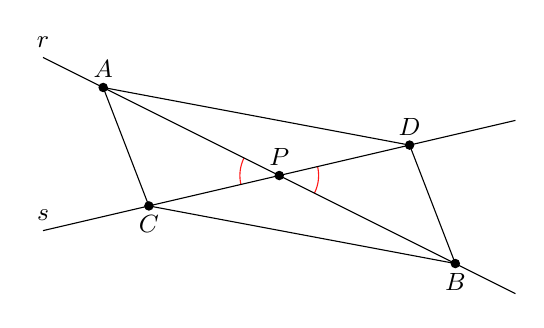
\begin{tikzpicture}[scale=1,font=\small]
\usetikzlibrary{calc}

\begin{scope}
\coordinate (s1) at (-3,-0.7);
\coordinate (s2) at (3,0.7);
\coordinate (r1) at (-3,1.5);
\coordinate (r2) at (3,-1.5);

\coordinate (p) at (intersection of r1--r2 and s1--s2);
\coordinate (a) at ($(p)!2.5cm!(r1)$);
\coordinate (b) at ($(p)!2.5cm!(r2)$);
\coordinate (c) at ($(p)!1.7cm!(s1)$);
\coordinate (d) at ($(p)!1.7cm!(s2)$);
\draw[fill] (a) circle (1.5pt) node[above] {$A$};
\draw[fill] (b) circle (1.5pt) node[below] {$B$};
\draw[fill] (c) circle (1.5pt) node[below] {$C$};
\draw[fill] (d) circle (1.5pt) node[above] {$D$};
\draw (a) -- (c) -- (b) -- (d) -- cycle;

\begin{scope}
\clip (a) -- (p) -- (c) -- cycle;
\draw[red!90] (p) circle (0.5);
%\node at ([shift={(0.7,0.3)}]p) {$\alpha$};
\end{scope}

\begin{scope}
\clip (b) -- (p) -- (d) -- cycle;
\draw[red!90] (p) circle (0.5);
%\node at ([shift={(0.7,0.3)}]p) {$\alpha$};
\end{scope}
\draw (s1) node[above] {$s$} -- (s2);
\draw (r1) node[above] {$r$} -- (r2);
\draw[fill] (p) circle (1.5pt) node[above] {$P$};

\end{scope}


\end{tikzpicture}

\caption{Esempio~\ref{esempio:2.1}}\label{fig:esempio2.1}
\end{figure}

\noindent Ipotesi: $r\cap s=P$, $AP\cong PB$, $CP\cong PD$.\tab\tab Tesi: $ACP\cong BDP$, $ADP\cong BPC$.

\begin{proof}
I triangoli $ACP$ e $BPD$ hanno: $AP\cong PB$ per ipotesi, $CP\cong PD$ per ipotesi, $A\widehat{P}C\cong B\widehat{P}D$ perché opposti al vertice. Pertanto sono congruenti per il 1\textsuperscript{o} criterio di congruenza dei triangoli.

Analogamente, i triangoli $ADP$ e $BPC$ hanno: \ldots\ldots\ldots\ldots\ldots\ldots\ldots
\end{proof}
\end{esempio}

\begin{esempio}\label{esempio:2.2}
Si considerino un segmento $AB$ ed il suo punto medio $M$. Si tracci una generica retta $r$ passante per $M$ e distinta dalla retta per $AB$. Si traccino inoltre due semirette di origine rispettivamente $A$ e $B$, situate nei due semipiani opposti rispetto alla retta per $AB$, che intersechino la retta $r$ rispettivamente in $C$ e in $D$ e che formino con la retta per $AB$ due angoli congruenti (vedi figura~\ref{fig:esempio2.2}). Detti $C$ e $D$ i rispettivi punti di intersezione delle due semirette con la retta $r$, dimostra che i triangoli $AMC$ e $BMD$ sono congruenti.

\begin{figure}[htb]
\centering% Copyright (c) 2015 Daniele Masini - d.masini.it@gmail.com

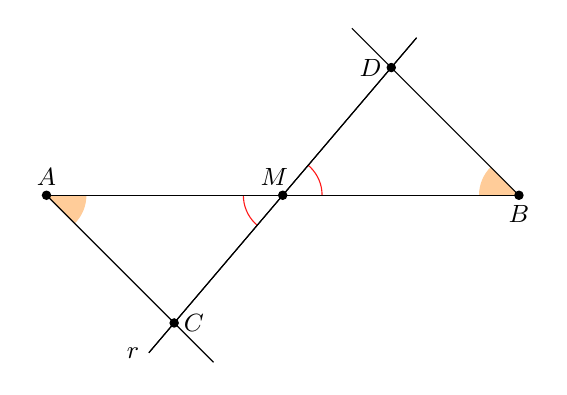
\begin{tikzpicture}[scale=1,font=\small]
\usetikzlibrary{calc}

\begin{scope}
\coordinate (a) at (-3,0);
\coordinate (b) at (3,0);
\coordinate (m) at (0,0);
\coordinate (r1) at (-1.7,-2);
\coordinate (r2) at (1.7,2);
\coordinate (s1) at ([shift={(135:3)}]b);
\coordinate (t1) at ([shift={(-45:3)}]a);
\coordinate (c) at (intersection of r1--r2 and a--t1);
\coordinate (d) at (intersection of r1--r2 and b--s1);

\begin{scope}
\clip (a) -- (m) -- (c) -- cycle;
\draw[fill,orange!40] (a) circle (0.5);
\draw[red!90] (m) circle (0.5);
%\node at ([shift={(0.7,0.3)}]p) {$\alpha$};
\end{scope}

\begin{scope}
\clip (b) -- (m) -- (d) -- cycle;
\draw[fill,orange!40] (b) circle (0.5);
\draw[red!90] (m) circle (0.5);
%\node at ([shift={(0.7,0.3)}]p) {$\alpha$};
\end{scope}

\draw[fill] (a) circle (1.5pt) node[above] {$A$};
\draw[fill] (b) circle (1.5pt) node[below] {$B$};
\draw[fill] (c) circle (1.5pt) node[right] {$C$};
\draw[fill] (d) circle (1.5pt) node[left] {$D$};
\draw (a) -- (b);
\draw (r1) -- (r2);
\draw (a) -- (t1);
\draw (b) -- (s1);

\draw (r1) node[left] {$r$} -- (r2);
\draw[fill] (m) circle (1.5pt) node[left = 3pt, above=0pt] {$M$};

\end{scope}


\end{tikzpicture}

\caption{Esempio~\ref{esempio:2.2}}\label{fig:esempio2.2}
\end{figure}

\noindent Ipotesi: $AM\cong MB$, $M\widehat{A}C\cong M\widehat{B}D$.\tab Tesi: $AMC\cong BMD$.

\begin{proof}
I segmenti $AM$ e $MB$ sono congruenti in quanto $M$ è il punto medio di $AB$, gli angoli di vertice $M$ sono congruenti perché opposti al vertice, gli angoli di vertici $A$ e $B$ sono congruenti per costruzione. Allora i triangoli $AMC$ e $BMD$ sono congruenti per il 2\textsuperscript{o} criterio di congruenza dei triangoli.
\end{proof}
\end{esempio}
\end{exrig}

\section{Teoremi del triangolo isoscele}\label{sect:teoremi_triangolo_isoscele}

Il \emph{triangolo isoscele} ha almeno due lati congruenti, l'eventuale lato non congruente si chiama \emph{base}, i due lati congruenti si dicono \emph{lati obliqui}.

Il \emph{triangolo equilatero} è un caso particolare di triangolo isoscele: si dice che \emph{il triangolo equilatero è isoscele rispetto a qualsiasi lato preso come base}.

\begin{teorema}[del triangolo isoscele {[}teorema diretto{]}]
In un triangolo isoscele gli angoli alla base sono congruenti.
\end{teorema}

\begin{figure}[htb]
\centering% Copyright (c) 2015 Daniele Masini - d.masini.it@gmail.com

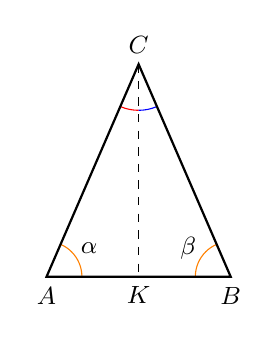
\begin{tikzpicture}[scale=0.9,font=\small]
\usetikzlibrary{calc}

\begin{scope}
\coordinate (a) at (-1.3,0);
\coordinate (b) at (1.3,0);
\coordinate (c) at (0,3);
\coordinate (k) at (0,0);

\begin{scope}
\clip (a) -- (b) -- (c) -- cycle;
\draw[orange] (a) circle (0.5);
\draw[orange] (b) circle (0.5);
\node at ([shift={(0.6,0.4)}]a) {$\alpha$};
\node at ([shift={(-0.6,0.4)}]b) {$\beta$};
\end{scope}

\begin{scope}
\clip (a) -- (c) -- (k) -- cycle;
\draw[red] (c) circle (0.65);
\end{scope}

\begin{scope}
\clip (b) -- (c) -- (k) -- cycle;
\draw[blue] (c) circle (0.65);
\end{scope}


\draw[thick] (a) node[below] {$A$} -- (b) node[below] {$B$} -- (c) node[above] {$C$} -- cycle;
\draw[dashed] (c) -- (k);
\node[below] at (k) {$K$};

\end{scope}


\end{tikzpicture}

\end{figure}

\noindent Ipotesi: $AC\cong BC$.\tab Tesi: $\alpha\cong \beta$.

\begin{proof}
Tracciamo la bisettrice $CK$ dell'angolo in $C$.
I triangoli $ACK$ e $BCK$ sono congruenti per il primo criterio, infatti hanno:
\begin{itemize*}
\item $AC\cong CB$ per ipotesi;
\item $CK$ lato in comune;
\item $A\widehat{C}K\cong B\widehat{C}K$ perché $CK$ è la bisettrice dell'angolo in $C$.
\end{itemize*}
Pertanto, essendo congruenti, i due triangoli hanno tutti gli elementi congruenti, in particolare l'angolo $\alpha$ (in $A$) è congruente all'angolo $\beta$ (in $B$).
\end{proof}

Il teorema precedente è invertibile, nel senso che è valido anche il teorema inverso, quello che si ottiene scambiando tra loro ipotesi e tesi.

\begin{teorema}[del triangolo isoscele {[}teorema inverso{]}]
Se un triangolo ha due angoli congruenti, allora è isoscele (rispetto al lato compreso tra gli angoli congruenti preso come base).
\end{teorema}

\begin{figure}[htb]
\centering% Copyright (c) 2015 Daniele Masini - d.masini.it@gmail.com

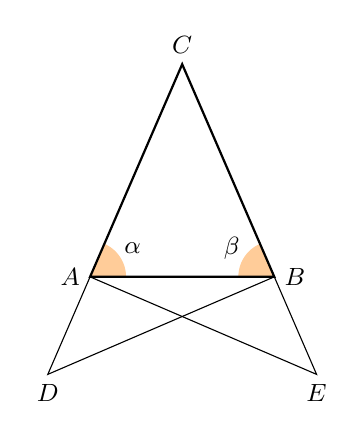
\begin{tikzpicture}[scale=0.9,font=\small]
\usetikzlibrary{calc}

\begin{scope}
\coordinate (a) at (-1.3,0);
\coordinate (b) at (1.3,0);
\coordinate (c) at (0,3);

\begin{scope}
\clip (a) -- (b) -- (c) -- cycle;
\draw[fill,orange!40] (a) circle (0.5);
\draw[fill,orange!40] (b) circle (0.5);
\node at ([shift={(0.6,0.4)}]a) {$\alpha$};
\node at ([shift={(-0.6,0.4)}]b) {$\beta$};
\end{scope}

\draw[thick] (a) node[left] {$A$} -- (b) node[right] {$B$} -- (c) node[above] {$C$} -- cycle;

\draw (a) -- ($(a)!-1.5cm!(c)$) node[below] {$D$} -- (b);
\draw (b) -- ($(b)!-1.5cm!(c)$) node[below] {$E$} -- (a);

\end{scope}


\end{tikzpicture}

\end{figure}

\noindent Ipotesi: $\alpha\cong \beta$.\tab Tesi: $AC\cong BC$.

\begin{proof}
Procediamo per passi, realizzando una costruzione che ci permetta di confrontare coppie di triangoli congruenti. Prolunghiamo i lati $AC$ e $BC$ dalla parte di $A$ e di $B$ rispettivamente, e sui prolungamenti prendiamo due punti $D$ ed $E$ in maniera tale che risulti $AD\cong BE$.

Osserviamo che i triangoli $ADB$ e $BAE$ risultano congruenti per il 1\textsuperscript{o} criterio, avendo in comune il lato $AB$ ed essendo $AD\cong BE$ per costruzione e $D\widehat{A}B\cong A\widehat{B}E$ perché adiacenti agli angoli $C\widehat{A}B$ e $C\widehat{B}A$ congruenti per ipotesi. Pertanto, tutti gli elementi dei due triangoli $ADB$ e $AEB$ sono ordinatamente congruenti, in particolare $DB\cong AE$, $A\widehat{D}B\cong B\widehat{E}A$ e $A\widehat{B}D\cong B\widehat{A}E$.

I triangoli $CDB$ e $CAE$ risultano dunque congruenti per il 2\textsuperscript{o} criterio poiché hanno $DB\cong AE$, $C\widehat{D}B\cong C\widehat{E}A$ per quanto appena dimostrato e $C\widehat{D}B\cong C\widehat{A}E$ perché somma di angoli rispettivamente congruenti: $C\widehat{B}D\cong C\widehat{B}A + A\widehat{B}D$ e $C\widehat{A}E\cong C\widehat{A}B + B\widehat{A}E$.

Pertanto, i restanti elementi dei due triangoli risultano ordinatamente congruenti, in particolare $CB\cong CA$, che è la tesi che volevamo dimostrare.
\end{proof}


Dai due teoremi precedenti seguono importanti proprietà, che qui riportiamo come corollari.

\begin{corollario}
Un triangolo equilatero è anche equiangolo.
\end{corollario}

\begin{proof}
Poiché un triangolo equilatero è isoscele rispetto a qualsiasi lato preso come base, la tesi segue dal teorema diretto del triangolo isoscele.
\end{proof}

\begin{corollario}
Se un triangolo è equiangolo allora è equilatero.
\end{corollario}

\begin{proof}
Possiamo confrontare gli angoli a due a due; risulteranno i lati congruenti a due a due in base al teorema inverso del triangolo isoscele.
\end{proof}

\begin{corollario}
Un triangolo scaleno non ha angoli congruenti.
\end{corollario}

\begin{proof}
Se per assurdo un triangolo scaleno avesse due angoli congruenti, allora risulterebbe isoscele, in base al teorema inverso del triangolo isoscele.
\end{proof}

\begin{corollario}
Se un triangolo non ha angoli congruenti allora è scaleno.
\end{corollario}

\begin{proof}
Se un triangolo non ha angoli tra loro congruenti non può essere isoscele.
\end{proof}

\begin{proposizione}[Proprietà del triangolo isoscele]
In ogni triangolo isoscele, la mediana relativa alla base è anche altezza e bisettrice.
\end{proposizione}
Nella figura, $CJ$ è per ipotesi la bisettrice dell'angolo al vertice $\gamma$ del triangolo $ABC$, $FK$ è la mediana relativa alla base $DE$ del triangolo $DEF$, $IL$ è l'altezza relativa alla base $GH$ del triangolo $GHI$.

\begin{figure}[htb]
\centering% Copyright (c) 2015 Daniele Masini - d.masini.it@gmail.com

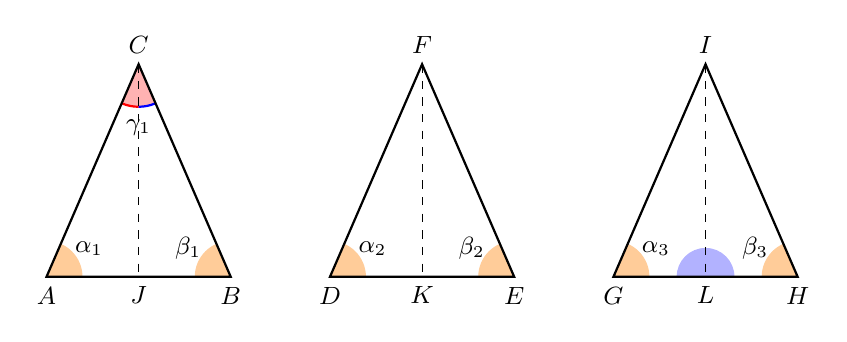
\begin{tikzpicture}[scale=0.9,font=\small]
\usetikzlibrary{calc}

\begin{scope}
\coordinate (a) at (-1.3,0);
\coordinate (b) at (1.3,0);
\coordinate (c) at (0,3);
\coordinate (j) at (0,0);

\begin{scope}
\clip (a) -- (b) -- (c) -- cycle;
\draw[fill,orange!40] (a) circle (0.5);
\draw[fill,orange!40] (b) circle (0.5);
\draw[fill,red!30] (c) circle (0.6);
\node at ([shift={(0.6,0.4)}]a) {$\alpha_1$};
\node at ([shift={(-0.6,0.4)}]b) {$\beta_1$};
\node at ([shift={(0,-0.9)}]c) {$\gamma_1$};
\end{scope}

\begin{scope}
\clip (a) -- (c) -- (j) -- cycle;
\draw[thick,red] (c) circle (0.6);
\end{scope}

\begin{scope}
\clip (b) -- (c) -- (j) -- cycle;
\draw[thick,blue] (c) circle (0.6);
\end{scope}

\draw[dashed] (c) -- (j) node[below] {$J$};
\draw[thick] (a) node[below] {$A$} -- (b) node[below] {$B$} -- (c) node[above] {$C$} -- cycle;

\end{scope}


\begin{scope}[xshift=4cm]
\coordinate (a) at (-1.3,0);
\coordinate (b) at (1.3,0);
\coordinate (c) at (0,3);
\coordinate (j) at (0,0);

\begin{scope}
\clip (a) -- (b) -- (c) -- cycle;
\draw[fill,orange!40] (a) circle (0.5);
\draw[fill,orange!40] (b) circle (0.5);
\node at ([shift={(0.6,0.4)}]a) {$\alpha_2$};
\node at ([shift={(-0.6,0.4)}]b) {$\beta_2$};
\end{scope}

\draw[dashed] (c) -- (j) node[below] {$K$};
\draw[thick] (a) node[below] {$D$} -- (b) node[below] {$E$} -- (c) node[above] {$F$} -- cycle;

\end{scope}

\begin{scope}[xshift=8cm]
\coordinate (a) at (-1.3,0);
\coordinate (b) at (1.3,0);
\coordinate (c) at (0,3);
\coordinate (j) at (0,0);

\begin{scope}
\clip (a) -- (b) -- (c) -- cycle;
\draw[fill,orange!40] (a) circle (0.5);
\draw[fill,orange!40] (b) circle (0.5);
\node at ([shift={(0.6,0.4)}]a) {$\alpha_3$};
\node at ([shift={(-0.6,0.4)}]b) {$\beta_3$};
\end{scope}

\begin{scope}
\clip (a) -- (b) -- (c) -- cycle;
\draw[fill,blue!30] (j) circle (0.4);
\end{scope}

\draw[dashed] (c) -- (j) node[below] {$L$};
\draw[thick] (a) node[below] {$G$} -- (b) node[below] {$H$} -- (c) node[above] {$I$} -- cycle;

\end{scope}

\end{tikzpicture}

\end{figure}

Dividiamo l'enunciato in tre parti:
\begin{enumeratea}
\item In un triangolo isoscele la bisettrice dell'angolo al vertice è anche altezza e mediana relativa alla base.
\item In un triangolo isoscele la mediana relativa alla base è anche bisettrice dell'angolo al vertice e altezza relativa alla base.
\item In un triangolo isoscele l'altezza relativa alla base è anche bisettrice dell'angolo al vertice e mediana relativa alla base.
\end{enumeratea}

Per ciascuna di esse scriviamo ipotesi e tesi.
\begin{enumeratea}
\item In $ABC$:	Ipotesi: $AC\cong CB$, $\alpha_1\cong \beta_1$, $A\widehat{C}J\cong B\widehat{C}J$. Tesi: $CJ\perp AB$, $AJ\perp JB$.
\item In $DEF$:	\,Ipotesi: $DF\cong FE$, $\alpha_2\cong \beta_2$, $DK\cong KE$.\tab Tesi: $FK\perp DE$, $D\widehat{F}K\cong E\widehat{F}K$.
\item In $GHI$:	\,Ipotesi: $IG\cong IH$, $\alpha_3\cong \beta_3$, $IL\cong GH$.\tab Tesi: $GL\perp LH$, $G\widehat{I}L\cong H\widehat{I}L$.
\end{enumeratea}

\begin{proof}
Avviamo la dimostrazione delle prime due parti, che lasciamo completare al lettore e rimandiamo al prossimo capitolo la dimostrazione della terza.

\begin{enumeratea}
\item I triangoli $AJC$ e $CJB$ sono congruenti per il 2\textsuperscript{o} criterio. Infatti hanno \ldots\ldots\ldots\ldots{}\\
Dunque $AJ\cong JB$ e $A\widehat{J}C\cong C\widehat{J}B$ che risultano pertanto retti in quanto adiacenti.  
\item I triangoli $DKF$ e $FKE$ sono congruenti per il 1\textsuperscript{o} criterio. Infatti hanno \ldots\ldots\ldots\ldots{}\\
Dunque $D\widehat{F}K\cong E\widehat{F}K$ e $F\widehat{K}D\cong F\widehat{K}E$ che risultano pertanto retti in quanto adiacenti.
\end{enumeratea}
\end{proof}

\section{Terzo criterio di congruenza dei triangoli}\label{sect:terzo_criterio_congruenza_triangoli}

\begin{teorema}[3\textsuperscript{o} criterio di congruenza dei triangoli]
Due triangoli sono congruenti se hanno congruenti le tre coppie di lati.
\end{teorema}

\begin{figure}[htb]
\centering\input{./lbr/chap02/fig011_3crit_cong_tri.pgf}
\end{figure}

\noindent Ipotesi: $AB\cong A'B'$, $BC\cong B'C'$, $AC\cong A'C'$.\tab Tesi: $ABC\cong A'B'C'$.

\begin{figure}[htb]
\centering% Copyright (c) 2015 Daniele Masini - d.masini.it@gmail.com

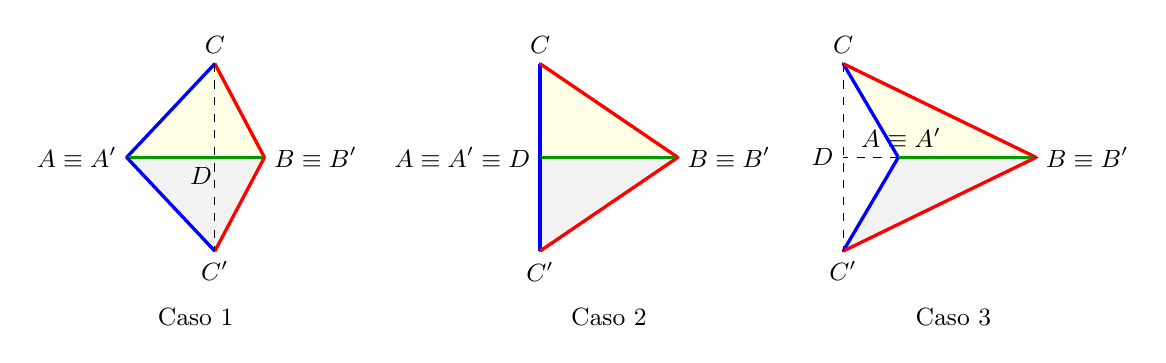
\begin{tikzpicture}[scale=.7,font=\small]
\usetikzlibrary{calc}

\begin{scope}
\coordinate (a) at (0,0);
\coordinate (c) at (1.6,1.7);
\coordinate (b) at (2.5,0);
\coordinate (c1) at (1.6,-1.7);

\draw[fill=gray!10] (a) -- (b) -- (c1) -- cycle;

\draw[fill=yellow!10] (a) -- (b) -- (c) -- cycle;
\draw (a) node[left] {$A\equiv A'$} -- (b) node[right] {$B\equiv B'$} -- (c) node[above] {$C$} -- cycle;
\draw[blue,very thick] (a) -- (c);
\draw[red,very thick] (c) -- (b);
\draw[green!60!black,very thick] (a) -- (b);

\draw[very thick,blue] (a) -- (c1);
\draw[very thick,red] (b) -- (c1);
\draw[dashed] (c) -- (c1) node[below] {$C'$};
\coordinate (d) at (intersection of a--b and c--c1);
\node[left=5pt, below] at (d) {$D$};

\node at (1.25,-2.9) {Caso 1};

\end{scope}


\begin{scope}[xshift=7.5cm]
\coordinate (a) at (0,0);
\coordinate (c) at (0,1.7);
\coordinate (b) at (2.5,0);
\coordinate (c1) at (0,-1.7);

\draw[fill=gray!10] (a) -- (b) -- (c1) -- cycle;

\draw[fill=yellow!10] (a) -- (b) -- (c) -- cycle;
\draw (a) node[left] {$A\equiv A'\equiv D$} -- (b) node[right] {$B\equiv B'$} -- (c) node[above] {$C$} -- cycle;
\draw[blue,very thick] (a) -- (c);
\draw[red,very thick] (c) -- (b);
\draw[green!60!black,very thick] (a) -- (b);

\draw[very thick,blue] (a) -- (c1);
\draw[very thick,red] (b) -- (c1) node[black,below] {$C'$};
\coordinate (d) at (intersection of a--b and c--c1);

\node at (1.25,-2.9) {Caso 2};

\end{scope}


\begin{scope}[xshift=14cm]
\coordinate (a) at (0,0);
\coordinate (c) at (-1,1.7);
\coordinate (b) at (2.5,0);
\coordinate (c1) at (-1,-1.7);

\draw[fill=gray!10] (a) -- (b) -- (c1) -- cycle;

\draw[fill=yellow!10] (a) -- (b) -- (c) -- cycle;
\draw (a) node[left=-1pt,above] {$A\equiv A'$} -- (b) node[right] {$B\equiv B'$} -- (c) node[above] {$C$} -- cycle;
\draw[blue,very thick] (a) -- (c);
\draw[red,very thick] (c) -- (b);
\draw[green!60!black,very thick] (a) -- (b);

\draw[very thick,blue] (a) -- (c1);
\draw[very thick,red] (b) -- (c1);
\draw[dashed] (c) -- (c1) node[below] {$C'$};
\coordinate (d) at (intersection of a--b and c--c1);
\draw[dashed] (a) -- (d);
%\node[left=5pt, below] at (d) {$D$};
\node[left] at (d) {$D$};

\node at (1,-2.9) {Caso 3};

\end{scope}

\end{tikzpicture}

\end{figure}

\begin{proof}
Abbiamo due triangoli, $ABC$ e $A'B'C'$, dei quali sappiamo che i lati dell'uno sono congruenti a quelli dell'altro. Ribaltiamo il triangolo $A'B'C'$ e portiamo il segmento $A'B'$ sul segmento $AB$ in modo che il punto $A'$ coincida con $A$, il punto $B'$ coincida con $B$ (ciò è possibile in quanto $AB\cong A'B'$) ed in modo che il punto $C'$ cada nel semipiano individuato dalla retta $AB$ opposto a quello in cui si trova $C$. Uniamo $C$ con $C'$. Viene fuori un disegno diverso a seconda che il punto di intersezione, che chiamiamo $D$, tra il segmento $CC'$ e la retta per $AB$, sia interno o esterno al segmento $AB$ oppure coincida con uno degli estremi ($A$ o $B$). Il punto $D$ esiste in ogni caso in quanto $C$ e $C'$ sono nei due semipiani opposti individuati dalla retta $AB$, pertanto il segmento $CC'$ deve necessariamente tagliare la retta per $AB$.

Caso 1: $D$ è interno ad $AB$.
Essendo $AC\cong A'C'$ e $CB\cong C'B'$, i triangoli $ACC'$ e $CC'B$ sono isosceli, entrambi sulla base $CC'$. Dunque, per il teorema (diretto) del triangolo isoscele, gli angoli alla base sono congruenti. Precisamente risulta: $A\widehat{C}C'\cong A\widehat{C'}C$ e $C'\widehat{C}B\cong C\widehat{C'}B$. Inoltre, $A\widehat{C}B\cong A\widehat{C'}B$ in quanto somme di angoli congruenti:
$A\widehat{C}B\cong A\widehat{C}D+D\widehat{C}B\cong A\widehat{C'}D+D\widehat{C'}B\cong A\widehat{C'}B$.
In conclusione $ABC$ e $ABC'$ sono congruenti per il primo criterio perché hanno: $AC\cong AC'$, $BC\cong BC'$, $A\widehat{C}B\cong A\widehat{C'}B$. 
Infine, poiché $ABC\cong ABC'$ e $ABC'\cong A'B'C'$ se ne deduce che $ABC\cong A'B'C'$.

Caso 2: $D$ coincide con uno dei due estremi (es.~$A$ e $A'$). 
Poiché per ipotesi $CB\cong C'B'$, il triangolo $CBC'$ è isoscele sulla base $CC'$, pertanto $A\widehat{C}B\cong A\widehat{C'}B$ in quanto angoli alla base di un triangolo isoscele. I triangoli $ABC$ e $ABC'$ sono quindi congruenti per il primo criterio perché hanno $AC\cong AC'$, $BC\cong BC'$ e $A\widehat{C}B\cong A\widehat{C'}B$. Infine, come per il caso precedente, poiché $ABC$ è congruente ad $ABC'$ e quest'ultimo è congruente ad $A'B'C'$ anche $ABC$ è congruente a $A'B'C'$.

Caso 3: $D$ cade esternamente al segmento $AB$.
Come nel caso 1, i triangoli $CAC'$ e $CBC'$ sono isosceli sulla base $CC'$, pertanto $A\widehat{C}C'\cong A\widehat{C'}C$ e $B\widehat{C}C'\cong B\widehat{C'}C$. Per differenza di angoli congruenti si ottiene che $A\widehat{C}B\cong A\widehat{C'}B$.
Infatti $A\widehat{C}B\cong D\widehat{C}B-D\widehat{C}A\cong D\widehat{C'}B-D\widehat{C'}A\cong A\widehat{C'}B$. Da ciò segue che i triangoli $ABC$ e $ABC'$ sono congruenti per il primo criterio in quanto hanno rispettivamente congruenti due lati e l'angolo tra essi compreso. Come per i casi precedenti, se $ABC$ è congruente a $ABC'$ è congruente anche a $A'B'C'$.
\end{proof}

\section{Congruenza dei poligoni}\label{sect:congruenza_poligoni}

Ricordiamo che due poligoni sono \emph{congruenti} se hanno lo stesso numero di lati ed hanno ``ordinatamente'' congruenti tutti i lati e tutti gli angoli corrispondenti.

Il seguente criterio di congruenza dei quadrilateri è una semplice applicazione del primo criterio di congruenza dei triangoli.
\begin{teorema}[1\textsuperscript{o} criterio di congruenza dei quadrilateri]
Due quadrilateri, aventi ordinatamente congruenti tre lati ed i due angoli tra essi compresi, sono congruenti.
\end{teorema}
Di conseguenza hanno ordinatamente congruenti anche il rimanente lato ed i rimanenti due angoli.

Conseguenza diretta del primo e del secondo criterio di congruenza dei triangoli è il seguente criterio.
\begin{teorema}[2\textsuperscript{o} criterio di congruenza dei quadrilateri]
Due quadrilateri, aventi ordinatamente congruenti due lati consecutivi e tre angoli (adiacenti ai due lati congruenti), sono congruenti.
\end{teorema}
Di conseguenza hanno ordinatamente congruenti anche il rimanente angolo ed i rimanenti due lati.

Conseguenza del primo e del terzo criterio di congruenza dei triangoli è il seguente criterio.
\begin{teorema}[3\textsuperscript{o} criterio di congruenza dei quadrilateri]
Due quadrilateri sono congruenti se hanno ordinatamente congruenti i quattro lati ed un angolo corrispondente.
\end{teorema}
Di conseguenza hanno ordinatamente congruenti anche i rimanenti tre angoli.

\begin{teorema}[Criteri di congruenza dei poligoni]
Due poligoni sono congruenti se hanno ordinatamente congruenti tutti i lati e tutti gli angoli compresi, tranne uno dei seguenti elementi su cui non si fa alcuna ipotesi:
\begin{itemize*}
\item due angoli consecutivi ed il lato compreso;
\item due lati consecutivi e l'angolo compreso;
\item tre angoli consecutivi.
\end{itemize*}
\end{teorema}

La dimostrazione di questi criteri è lasciata al lettore che potrà esercitarsi applicando i tre criteri di congruenza dei triangoli.


\newpage

% (c) 2014 Daniele Masini - d.masini.it@gmail.com
\section{Esercizi}

\begin{esercizio}
\label{ese:2.1}
In base alla figura a lato rispondi alle seguenti domande\\
\begin{minipage}{.7\linewidth}
\begin{enumeratea}
\item Il lato $AB$ si oppone all'angolo \ldots\ldots\ldots
\item L'angolo $\alpha$ si oppone al lato \ldots\ldots\ldots
\item L'angolo di vertice $C$ si chiama \ldots\ldots\ldots
\item L'angolo $\gamma$ è adiacente ai lati \ldots\ldots{} e \ldots\ldots
\item I lati $AB$ e $BC$ sono adiacenti all'angolo \ldots\ldots
\item I lati $AC$ e $AB$ formano l'angolo \ldots\ldots
\item Traccia l'angolo esterno al triangolo nel vertice $A$
\item Traccia la bisettrice dell'angolo $\beta$
\item Traccia l'altezza relativa alla base $AB$
\item Traccia la mediana relativa al lato $BC$
\end{enumeratea}
\end{minipage}\hfil
\begin{minipage}{.3\linewidth}
%\begin{wrapfigure}{r}{0pt}
  \centering
    % Copyright (c) 2015 Daniele Masini - d.masini.it@gmail.com

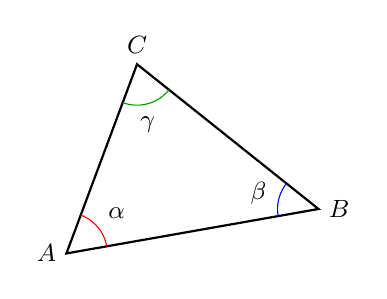
\begin{tikzpicture}[scale=1.3,font=\small]
\usetikzlibrary{calc}

\begin{scope}[rotate=10]
\coordinate (a) at (0,0);
\coordinate (c) at (1,1.7);
\coordinate (b) at (2.5,0);

\draw[thick] (b) node[right] {$B$} -- (c) node[above] {$C$} -- (a) node[left] {$A$} -- cycle;

\begin{scope}
\clip (a) -- (b) -- (c) -- cycle;
\draw[red] (a) circle (0.4);
\node at ([shift={(.55,.3)}]a) {$\alpha$};
\draw[blue] (b) circle (0.4);
\node at ([shift={(-.55,.25)}]b) {$\beta$};
\draw[green!60!black] (c) circle (0.4);
\node at ([shift={(0,-.6)}]c) {$\gamma$};
\end{scope}

\end{scope}

\end{tikzpicture}

%\end{wrapfigure}
\end{minipage}
\end{esercizio}

\begin{esercizio}
\label{ese:2.2}
Disegna un segmento $AB$, quindi disegna i triangoli $ABC$ e $ABD$ che hanno la base $AB$ in comune.
\end{esercizio}

\begin{esercizio}
\label{ese:2.3}
Disegna le tre altezze di ciascuno dei triangoli nella figura~\ref{fig:ese2.3}.
\end{esercizio}

\begin{figure}[htb]
\centering% Copyright (c) 2015 Daniele Masini - d.masini.it@gmail.com

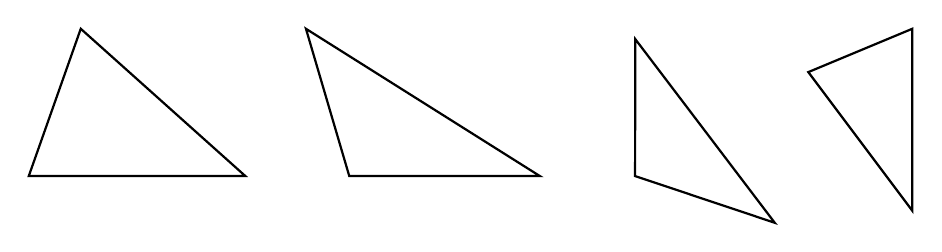
\begin{tikzpicture}[scale=1.1,font=\small]
\usetikzlibrary{calc}

\begin{scope}
\coordinate (a) at (0,0);
\coordinate (c) at (0.6,1.7);
\coordinate (b) at (2.5,0);
\draw[thick] (b)-- (c) -- (a) -- cycle;
\end{scope}

\begin{scope}[xshift=3.7cm]
\coordinate (a) at (0,0);
\coordinate (c) at (-.5,1.7);
\coordinate (b) at (2.2,0);
\draw[thick] (b)-- (c) -- (a) -- cycle;
\end{scope}

\begin{scope}[xshift=7cm, rotate=-18.5]
\coordinate (a) at (0,0);
\coordinate (c) at (-.5,1.5);
\coordinate (b) at (1.7,0);
\draw[thick] (b)-- (c) -- (a) -- cycle;
\end{scope}

\begin{scope}[xshift=9cm]
\coordinate (a) at (0,1.2);
\coordinate (c) at (1.2,1.7);
\coordinate (b) at (1.2,-0.4);
\draw[thick] (b)-- (c) -- (a) -- cycle;
\end{scope}


\end{tikzpicture}

\caption{Esercizio~\ref{ese:2.3}}\label{fig:ese2.3}
\end{figure}

\begin{esercizio}
\label{ese:2.4}
Per ciascuna delle coppie di triangoli a lato indica se sono congruenti ed eventualmente per quale criterio.\\
\begin{minipage}{.5\linewidth}
\begin{enumeratea}
\item Si sa che sono congruenti i lati $AB$ con $A'B'$ e $AC$ con $A'C'$, l'angolo $\widehat{A}$ con l'angolo $\widehat{A'}$.\\
I triangoli sono congruenti?\tab	Sì\quad	No\\
Se sì, per il \ldots\ldots\ldots\ldots\ldots\ldots\ldots\ldots

\item Si sa che sono congruenti i lati $AB$ con $A'B'$ e gli angoli $\widehat{A}$ con $\widehat{B'}$ e $\widehat{B}$ con $\widehat{A'}$.\\
I triangoli sono congruenti?\tab	Sì\quad	No\\
Se sì, per il \ldots\ldots\ldots\ldots\ldots\ldots\ldots\ldots

\item Si sa che sono congruenti i lati $AB$ con $A'B'$ e $BC$ con $A'C'$, l'angolo $\widehat{A}$ con $\widehat{A'}$.\\
I triangoli sono congruenti?\tab	Sì\quad	No\\
Se sì, per il \ldots\ldots\ldots\ldots\ldots\ldots\ldots\ldots
\end{enumeratea}
\end{minipage}\hfil
\begin{minipage}{.4\linewidth}
  \centering
    % Copyright (c) 2015 Daniele Masini - d.masini.it@gmail.com

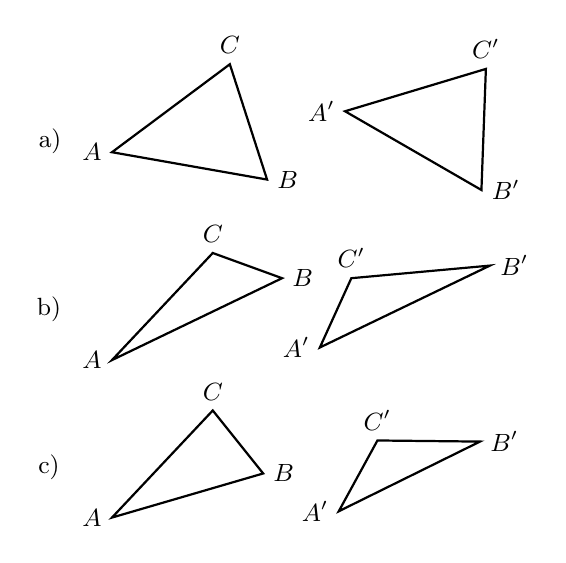
\begin{tikzpicture}[scale=0.8,font=\small]
\usetikzlibrary{calc}

\begin{scope}[rotate=-10]
\coordinate (a) at (0,0);
\coordinate (c) at (1.6,1.7);
\coordinate (b) at (2.5,0);
\draw[thick] (b) node[right] {$B$} -- (c) node[above] {$C$} -- (a) node[left] {$A$} -- cycle;
\node at (-1,0) {a)};
\end{scope}

\begin{scope}[xshift=3.7cm,yshift=0.65cm,rotate=-30]
\coordinate (a) at (0,0);
\coordinate (c) at (1.6,1.7);
\coordinate (b) at (2.5,0);
\draw[thick] (b) node[right] {$B'$} -- (c) node[above] {$C'$} -- (a) node[left] {$A'$} -- cycle;
\end{scope}

\begin{scope}[yshift=-3.3cm]
\coordinate (a) at (0,0);
\coordinate (c) at (1.6,1.7);
\coordinate (b) at (2.7,1.3);
\draw[thick] (b) node[right] {$B$} -- (c) node[above] {$C$} -- (a) node[left] {$A$} -- cycle;
\node at (-1,0.8) {b)};
\end{scope}

\begin{scope}[xshift=3.3cm,yshift=-3.1cm]
\coordinate (a) at (0,0);
\coordinate (c) at (0.5,1.1);
\coordinate (b) at (2.7,1.3);
\draw[thick] (b) node[right] {$B'$} -- (c) node[above] {$C'$} -- (a) node[left] {$A'$} -- cycle;
\end{scope}

\begin{scope}[yshift=-5.8cm]
\coordinate (a) at (0,0);
\coordinate (c) at (1.6,1.7);
\coordinate (b) at (2.4,0.7);
\draw[thick] (b) node[right] {$B$} -- (c) node[above] {$C$} -- (a) node[left] {$A$} -- cycle;
\node at (-1,0.8) {c)};
\end{scope}

\begin{scope}[xshift=3.6cm,yshift=-5.7cm,rotate=10]
\coordinate (a) at (0,0);
\coordinate (c) at (0.8,1);
\coordinate (b) at (2.4,0.7);
\draw[thick] (b) node[right] {$B'$} -- (c) node[above] {$C'$} -- (a) node[left] {$A'$} -- cycle;
\end{scope}


\end{tikzpicture}

\end{minipage}
\end{esercizio}

\begin{multicols}{2}

\subsubsection*{Dimostra le seguenti affermazioni, utilizzando il 1\textsuperscript{o} e il 2\textsuperscript{o} criterio di congruenza dei triangoli.}

\begin{esercizio}
\label{ese:2.5}
In un triangolo $ABC$ prolunga la mediana $AM$ di un segmento $MD$ congruente a $MA$. Dimostra che il triangolo $AMC$ è congruente al triangolo $BMD$ e che il triangolo $ABM$ è congruente al triangolo $CMD$.
\end{esercizio}

\begin{esercizio}
\label{ese:2.6}
Due triangoli $ABC$ e $DEF$ hanno il lati $AB$ e $DE$ congruenti, hanno inoltre gli angoli esterni ai vertici $A$ e $B$ rispettivamente congruenti agli angoli esterni ai vertici $D$ e $E$. Dimostra che i due triangoli sono congruenti.
\end{esercizio}

\begin{esercizio}
\label{ese:2.7}
Si consideri il segmento $AB$ e per il suo punto medio $M$ si tracci una retta $r$ qualsiasi. Su tale semiretta, da parti opposte rispetto a $AB$, si prendano due punti $S$ e $T$ tali che $SM\cong MT$. Dimostrare che i triangoli $AMS$ e $TMB$ sono congruenti.
\end{esercizio}

\begin{esercizio}
\label{ese:2.8}
Due triangoli rettangoli sono congruenti se hanno rispettivamente congruenti i due cateti.
\end{esercizio}

\begin{esercizio}
\label{ese:2.9}
Due triangoli rettangoli sono congruenti se hanno congruenti un cateto e l'angolo acuto adiacente ad esso.
\end{esercizio}

\begin{esercizio}
\label{ese:2.10}
Due triangoli isosceli sono congruenti se hanno congruenti tra loro l'angolo al vertice e i due lati obliqui.
\end{esercizio}

\begin{esercizio}
\label{ese:2.11}
Nel triangolo isoscele $ABC$, di base $BC$, prolunga la bisettrice $AD$ di un segmento $DE$. Dimostra che $AE$ è bisettrice dell'angolo $B\widehat{E}C$.
\end{esercizio}

\begin{esercizio}
\label{ese:2.12}
Dati due triangoli congruenti $ABC$ e $A'B'C'$, si considerino sui lati $AC$ e $A'C'$ due punti $D$ e $D'$ tali che $DC\cong D'C'$.  Dimostrare che $DB\cong D'B'$.
\end{esercizio}

\begin{esercizio}
\label{ese:2.13}
Siano $ABC$ e $DEF$ due triangoli congruenti. Sui lati congruenti $AB$ e $DE$ prendi il punto $G$ su $AB$ e $H$ su $DE$, in modo che $AG\cong DH$. Dimostra che anche $GC$ è congruente ad $HF$.
\end{esercizio}

\begin{esercizio}
\label{ese:2.14}
In un triangolo $ABC$, sul prolungamento del lato $AB$, dalla parte di $B$, prendi un punto $D$ tale che $BD\cong AB$, analogamente sul prolungamento del lato $CB$, dalla parte di $B$, prendi un punto $E$ tale che $EB\cong BC$. Dimostra che la mediana $BM$ del triangolo $ABC$ è allineata con la mediana $BN$ del triangolo $DBE$, ossia che l'angolo formato dalle due mediane è un angolo piatto.
\end{esercizio}

\begin{esercizio}
\label{ese:2.15}
Del triangolo $ABC$ prolunga il lato $AB$ di un segmento $BD$ congruente a $BC$, analogamente prolunga il lato $CB$ di un segmento $BE$ congruente ad $AB$. Traccia la bisettrice dell'angolo $A\widehat{B}C$ e sia $F$ la sua intersezione con $AC$. Traccia la bisettrice dell'angolo $D\widehat{B}E$ e chiama $G$ la sua intersezione con $DE$. Dimostra che $BF\cong BG$.
\end{esercizio}

\begin{esercizio}
\label{ese:2.16}
Nel triangolo $ABC$ traccia la bisettrice $AD$ dell'angolo in $A$. Con origine in $D$ traccia due semirette che incontrano rispettivamente $AC$ in $E$ e $AB$ in $F$, in modo che $A\widehat{D}F\cong A\widehat{D}E$. Dimostra che il triangolo $AFE$ è un triangolo isoscele.
\end{esercizio}

\begin{esercizio}
\label{ese:2.17}
Nel triangolo $ABC$ con $AC<AB$ traccia la bisettrice $AD$ dell'angolo in $A$. Per il punto $D$ traccia la perpendicolare alla bisettrice $AD$. Detti $E$ ed $F$ i punti in cui la perpendicolare incontra rispettivamente i lati $AC$ e $AB$, dimostra che $AF\cong AE$.
\end{esercizio}

\begin{esercizio}
\label{ese:2.18}
Sui prolungamenti oltre $A$ del lato $AC$, oltre $B$ del lato $AB$ e oltre $C$ del lato $BC$ di un triangolo equilatero $ABC$ si considerino i segmenti congruenti $AA'$, $BB'$, $CC'$. Dimostrare che il triangolo $A'B'C'$ è ancora equilatero.
\end{esercizio}

\begin{esercizio}
\label{ese:2.19}
Dato l'angolo convesso $b\widehat{A}c$ si considerino su $b$ i due punti $B$ e $B'$ e su $c$ i punti $C$ e $C'$, tali che $AB$ e $AB'$ siano rispettivamente congruenti con $AC$ e $AC'$. Dimostrare che $BB'$ e $BC'$ sono rispettivamente congruenti con $CC'$ e $B'C$.
\end{esercizio}

\begin{esercizio}
\label{ese:2.20}
Dato un segmento $AB$, condurre per il suo punto medio $M$ una qualsiasi retta $r$ e considerare su di essa, da parti opposte rispetto ad $AB$, due segmenti congruenti $MC$ e $MD$. Dimostrare che i triangoli $AMC$ e $BMD$ sono congruenti.
\end{esercizio}

\begin{esercizio}
\label{ese:2.21}
Sui lati dell'angolo $X\widehat{O}Y$ si considerino i punto $A$ e $B$ tali che $OA\cong OB$. Sia $H$ un punto della bisettrice dell'angolo tale che $OH<OA$. Siano $T$ il punto di intersezione di $AH$ con $OY$ e $S$ il punto di intersezione di $BH$ con $OX$. Dimostrare che $AH\cong HB$ e $SH\cong HT$.
\end{esercizio}

\begin{esercizio}
\label{ese:2.22}
Si consideri un punto $O$ interno al triangolo $ABC$ e si congiunga tale punto con i vertici $A$ e $B$ del triangolo. Si prolunghino i segmenti $AO$ e $BO$ oltre $O$ di due segmenti $OA'$ e $OB'$ rispettivamente congruenti ai suddetti segmenti. Dimostrare che i segmenti $AB$ e $A'B'$ sono congruenti.
\end{esercizio}

\begin{esercizio}
\label{ese:2.23}
Si considerino i triangoli congruenti $ABC$ e $A'B'C'$ e si prolunghino i lati $AB$ e $A'B'$ di due segmenti $BP$ e $B'P'$ tra loro congruenti. Si prolunghino inoltre i lati $AC$ e $A'C'$ di due segmenti $CQ$ e $C'Q'$ tra loro congruenti. Si dimostri che sono congruenti i triangoli $APQ$ e $A'P'Q'$ e che $CP\cong C'P'$, $QB\cong Q'B'$.
\end{esercizio}

\begin{esercizio}
\label{ese:2.24}
Sui lati $a$ e $b$ di un angolo di vertice $O$ prendi i punti $A$ e $B$ sulla semiretta $a$ e i punti $C$ e $D$ sulla semiretta $b$, in modo che $OA\cong OC$ e $AB\cong CD$. Sia $E$ il punto di intersezione di $AD$ con $BC$. Dimostra che sono congruenti i triangoli $ABE$ e $CDE$.
\end{esercizio}

\begin{esercizio}
\label{ese:2.25}
Sia $C$ un punto della bisettrice dell'angolo convesso $a\widehat{O}b$, $A$ un punto sul lato $a$ e $B$ un punto sul lato $b$, tali che $OA\cong OB$. Dimostra che i triangoli $BCO$ e $ACO$ sono congruenti.
\end{esercizio}

\begin{esercizio}
\label{ese:2.26}
Dato un triangolo $ABC$, traccia la parallela ad $AC$ passante per $B$ e la parallela a $BC$ passante per $A$. Indica con $D$ il punto di intersezione delle due rette tracciate. Dimostra che i triangoli $ABC$ e $ABD$ sono congruenti.
\end{esercizio}

\subsubsection*{Dimostra le seguenti affermazioni sui triangoli isosceli.}

\begin{esercizio}
\label{ese:2.27}
In un triangolo isoscele le mediane relative ai lati congruenti sono congruenti. 
\end{esercizio}

\begin{esercizio}
\label{ese:2.28}
In un triangolo isoscele le bisettrici degli angoli alla base sono congruenti. 
\end{esercizio}

\begin{esercizio}
\label{ese:2.29}
Due triangoli isosceli sono congruenti se hanno rispettivamente congruenti l'angolo al vertice e uno dei lati obliqui.
\end{esercizio}

\begin{esercizio}
\label{ese:2.30}
Due triangoli isosceli sono congruenti se hanno rispettivamente congruenti la base e uno degli angoli ad essa adiacenti.
\end{esercizio}

\begin{esercizio}
\label{ese:2.31}
Due triangoli isosceli sono congruenti se hanno rispettivamente congruenti la base e la bisettrice dell'angolo al vertice.
\end{esercizio}

\begin{esercizio}
\label{ese:2.32}
Due triangoli isosceli sono congruenti se hanno rispettivamente congruenti gli angoli al vertice e due lati corrispondenti qualsiasi.
\end{esercizio}

\begin{esercizio}
\label{ese:2.33}
Sia $P$ il punto di intersezione delle bisettrici degli angoli alla base $AB$ di un triangolo isoscele $ABC$. Dimostra che anche $APB$ è isoscele.
\end{esercizio}

\begin{esercizio}
\label{ese:2.34}
In un triangolo isoscele $ABC$ di base $AB$ e vertice $C$, prendi su $AC$ un punto $M$ e su $BC$ un punto $N$ in modo che $CM\cong CN$. Quali delle seguenti coppie di triangoli sono congruenti? Dimostralo.
\begin{multicols}{2}
\begin{enumeratea}
\item $ACN$ e $ANB$
\item $ACN$ e $BCM$
\item $ABN$ e $ABM$
\item $ABC$ e $MNC$
\end{enumeratea}
\end{multicols}
\end{esercizio}

\begin{esercizio}
\label{ese:2.35}
In un triangolo isoscele $ABC$ di base $AB$ e vertice $C$, indica con $M$ il punto medio di $AC$, con $N$ il punto medio di $CB$ e con $H$ il punto medio di $AB$. Quali delle seguenti coppie di triangoli sono congruenti? Dimostralo.
\begin{multicols}{2}
\begin{enumeratea}
\item $AMH$ e $HNB$
\item $MNH$ e $MNC$
\item $AMH$ e $MCN$
\end{enumeratea}
\end{multicols}
\end{esercizio}

\begin{esercizio}
\label{ese:2.36}
Sui lati $AC$ e $CB$ del triangolo isoscele $ABC$ di base $AB$ considera rispettivamente due punti $D$ ed $E$ tali che $CD\cong CE$. Dimostra che i triangoli $ADB$ e $AEB$ sono congruenti. Detto $P$ il punto di intersezione tra $AE$ e $DB$, dimostrare che $ABP$ e $DPE$ sono triangoli isosceli.
\end{esercizio}

\begin{esercizio}
\label{ese:2.37}
In un triangolo isoscele $ABC$ di base $AB$ e vertice $C$ prolunga la base $AB$, dalla parte di $A$ di un segmento $AD$ e dalla parte di $B$ di un segmento $BE$ congruente ad $AD$. Dimostra che anche il triangolo $DEC$ è isoscele.
\end{esercizio}

\begin{esercizio}
\label{ese:2.38}
Nel triangolo isoscele $ABC$ di base $BC$, prendi sul prolungamento di $BC$ due segmenti congruenti $BQ$ e $CP$. Dimostra che $APB$ è isoscele.
\end{esercizio}

\begin{esercizio}
\label{ese:2.39}
Due triangoli isosceli $ABC$ e $ABD$ hanno in comune la base $AB$, i vertici $C$ e $D$ sono situati da parti opposte rispetto alla base $AB$. Dimostra che la retta per $CD$ è bisettrice dell'angolo in $C$.
\end{esercizio}

\begin{esercizio}
\label{ese:2.40}
In un triangolo isoscele $ABC$ di base $AB$ e vertice $C$ traccia le bisettrici $BD$ all'angolo in $B$ e $AE$ all'angolo in $A$. Dimostra che $BD\cong AE$. Detto $O$ il punto di intersezione delle bisettrici dimostra che $AOB$ è isoscele. Dimostra che il triangolo $ADO$ è congruente al triangolo $BEO$.
\end{esercizio}

\begin{esercizio}
\label{ese:2.41}
In un triangolo isoscele $ABC$ di base $AB$ e vertice $C$ prolunga, dalla parte di $C$ la bisettrice $CD$ dell'angolo in $C$ di un segmento $CE$. Dimostra che $ED$ è bisettrice dell'angolo $A\widehat{E}D$.
\end{esercizio}

\begin{esercizio}
\label{ese:2.42}
In un triangolo isoscele $ABC$ di base $AB$ e vertice $C$ prendi su $AC$ un punto $D$ e su $BC$ il punto $E$ tali che $AD\cong BE$. Detto $O$ il punto di intersezione di $AE$ con $BD$, dimostra che $AOB$ è isoscele.
\end{esercizio}

\begin{esercizio}
\label{ese:2.43}
In un triangolo $ABC$ sia $M$ il punto medio di $AB$. Traccia la mediana $CM$ e prolungala dalla parte di $M$ di un segmento $MD$ congruente a $CM$. Dopo aver dimostrato che il triangolo $AMC$ è congruente a $BMD$, dimostra che se $CM$ è bisettrice dell'angolo in $C$ allora $ABC$ è isoscele.
\end{esercizio}

\begin{esercizio}
\label{ese:2.44}
In un triangolo isoscele $ABC$ di base $AB$ e vertice $C$, prendi su $AC$ un punto $D$ e su $CB$ un punto $E$ in modo che $CD\cong CE$. Dimostra che il triangolo $DME$, dove $M$ è il punto medio della base $AB$, è isoscele.
\end{esercizio}

\begin{esercizio}
\label{ese:2.45}
Due triangoli isoscele hanno in comune la base, dimostra che la retta che unisce i vertici dei due triangoli divide la base a metà.
\end{esercizio}

\begin{esercizio}
\label{ese:2.46}
In un triangolo isoscele $ABC$ di base $AB$ e vertice $C$, si ha che $AC\cong CB\cong 2\cdot AB$. Indica con $M$ il punto medio di $AC$ e $N$ il punto medio di $BC$, $P$ il punto di intersezione di $BM$ con $AN$. Individua tutti i triangoli isosceli che si vengono a formare. Dimostra che $ACN$ è congruente a $BCM$, che $ABP$ è isoscele, che $P$ appartiene all'altezza $CH$ del triangolo.
\end{esercizio}

\begin{esercizio}
\label{ese:2.47}
Sia dato il triangolo $ABC$ e sia $M$ il punto medio del lato $AB$. Si prolunghi $CM$ di un segmento $MD\cong CM$. Dimostrare che $A\widehat{C}B\cong A\widehat{D}B$.
\end{esercizio}

\begin{esercizio}
\label{ese:2.48}
Si prolunghino i lati $AC$ e $CB$ del triangolo isoscele $ABC$ rispettivamente di due segmenti $CP$ e $CQ$ tra loro congruenti. Dimostrare che $A\widehat{Q}B\cong A\widehat{P}Q$ e che $A\widehat{B}P\cong Q\widehat{A}B$.
\end{esercizio}

\begin{esercizio}
\label{ese:2.49}
Sulla base $AB$ di un triangolo isoscele $ABC$ prendi i punti $M$ e $N$ tali che $AM<AN$ e $AM\cong NB$. Dimostra che $CMN$ è isoscele.
\end{esercizio}

\begin{esercizio}
\label{ese:2.50}
Sia $D$ il punto di intersezione delle bisettrici degli angoli alla base di un triangolo isoscele $ABC$ di vertice $A$. Dimostra che $BDC$ è isoscele.
\end{esercizio}

\begin{esercizio}
\label{ese:2.51}
Nel triangolo isoscele $ABC$ di base $BC$ prolunga $AB$ di un segmento $BD$ e $AC$ di un segmento $CE$ in modo che $DE\cong CE$. Dimostra che $BE\cong DC$.
\end{esercizio}

\begin{esercizio}
\label{ese:2.52}
Sia $ABC$ un triangolo isoscele con $AB\cong AC$. Sui lati obliqui $AB$ e $AC$ costruisci, esternamente al triangolo, i triangoli equilateri $ABD$ e $ACE$. Congiungi $B$ con $E$ e $C$ con $D$. Detto $F$ il punto di intersezione di $DC$ e $BE$, dimostra che $BFC$ è isoscele.
\end{esercizio}

\subsubsection*{Esercizi sui criteri di congruenza dei triangoli e sui triangoli isosceli.}

\begin{esercizio}
\label{ese:2.53}
Due triangoli sono congruenti se hanno
\begin{enumeratea}
\item tre lati congruenti \hfill\boxV\quad\boxF
\item tre angoli congruenti \hfill\boxV\quad\boxF
\item due lati e l'angolo compreso congruenti\tab\hfill\boxV\quad\boxF
\item due angoli e il lato in comune congruenti\tab\hfill\boxV\quad\boxF
\item un lato e l'angolo opposto congruenti\tab\tab\hfill\boxV\quad\boxF
\end{enumeratea}
\end{esercizio}

\begin{esercizio}
\label{ese:2.54}
Prolunga nello stesso verso i lati di un triangolo equilatero di tre segmenti tra loro congruenti. Dimostra che il triangolo ottenuto congiungendo gli estremi dei segmenti aggiunti è equilatero.
\end{esercizio}

\begin{esercizio}
\label{ese:2.55}
Due triangoli equilateri sono congruenti se hanno lo stesso perimetro.
\end{esercizio}

\begin{esercizio}
\label{ese:2.56}
Dimostra che due triangoli equilateri che hanno in comune la base sono congruenti.
\end{esercizio}

\begin{esercizio}
\label{ese:2.57}
Se in due triangoli sono congruenti due coppie di lati e la mediana relativa ad uno di essi, allora i due triangoli sono congruenti.
\end{esercizio}

\begin{esercizio}
\label{ese:2.58}
Se in due triangoli sono congruenti due coppie di lati e la bisettrice relativa ad uno di essi, allora i due triangoli sono congruenti.
\end{esercizio}

\begin{esercizio}
\label{ese:2.59}
Due triangoli isosceli sono congruenti se hanno rispettivamente congruenti la base e un altro lato.
\end{esercizio}

\begin{esercizio}
\label{ese:2.60}
Se due triangoli hanno congruenti due lati e la mediana relativa a uno di essi allora sono congruenti.
\end{esercizio}

\begin{esercizio}
\label{ese:2.61}
In un triangolo se la bisettrice di un angolo è anche meddiana allora il triangolo è isoscele.
\end{esercizio}

\begin{esercizio}
\label{ese:2.62}
In un triangolo isoscele $ABC$ di base $BC$ e vertice $A$ prendi un punto $D$ sul lato $AB$ e un punto $E$ sul lato $AC$, in modo che $BD\cong EC$, unisci $C$ con $D$ e $B$ con $E$. Sia $F=BE\cap DC$. Dimostra che i triangoli $BFA$ e $CFA$ sono congruenti.
\end{esercizio}

\begin{esercizio}
\label{ese:2.63}
Dimostra che, prolungando i lati congruenti $AB$ e $AC$ di un triangolo isoscele di due segmenti congruenti rispettivamente $AP$ e $AQ$, si ha che $BQ\cong PC$.
\end{esercizio}

\begin{esercizio}
\label{ese:2.64}
In un triangolo isoscele $ABC$ di base $BC$ e vertice $A$, prolunga il lato $AB$ di un segmento $BD$ e il lato $AC$ di un segmento $CE$ in modo che $BD\cong CE$, prolunga la base $BC$ di un segmento $BG$, dalla parte di $B$, e di un segmento $CF$ dalla parte di $C$, in modo che $BG\cong CF$. Dimostra che sono congruenti i triangoli $ADG$ e $AEF$.
\end{esercizio}

\begin{esercizio}
\label{ese:2.65}
In un triangolo scaleno $ABC$ sia $AC>BC$. Prolunga $BC$, dalla parte di $C$, di un segmento $CD$ congruente ad $AC$ e prolunga $AC$, dalla parte di $C$, di un segmento $CE$ congruente a $BC$. Detto $H$ il punto di intersezione della retta per $AB$ con la retta per $DE$, dimostra che $AH\cong DH$.
\end{esercizio}

\begin{esercizio}
\label{ese:2.66}
In un triangolo isoscele $ABC$ di base $BC$ e vertice $A$, prolunga il lato $AB$ di un segmento $BD$ e il lato $AC$ di un segmento $CE$ in modo che $BD\cong CE$. Unisci $D$ con $C$ e prolunga il segmento $DC$, dalla parte di $C$ di un segmento $CF$. Unisci $E$ con $B$ e prolunga il segmento $EB$ dalla parte di $B$ di un segmento $BG\cong CF$. Dimostra che i triangoli $AGD$ e $AFE$ sono congruenti.
\end{esercizio}

\begin{esercizio}
\label{ese:2.67}
Dato il triangolo convesso non piatto $a\widehat{O}b$ si prenda un punto $A$ sul lato $Oa$ e un punto $B$ sul lato $Ob$, in modo che $OA\cong OB$. Sia $M$ il punto medio di $OA$ e $N$ il punto medio di $OB$, congiungi $A$ con $N$ e $B$ con $M$, indica con $P$ in punto di intersezione. Dimostra che sono congruenti i triangoli $OBC$ e $OAD$ e i triangoli $AOP$ e $OPB$.
\end{esercizio}

\begin{esercizio}
\label{ese:2.68}
Nel triangolo isoscele $ABC$ di base $AB$ e vertice $C$, prendi un punto $D$ sulla bisettrice $CH$ dell'angolo al vertice $C$, indica con $E$ il punto di intersezione della retta $AD$ con $BC$ e $F$ il punto di intersezione di $BD$ con $AC$. Dimostra che i triangoli $FDA$ e $EDB$ sono congruenti.
\end{esercizio}

\begin{esercizio}
\label{ese:2.69}
Siano $ABC$ e $ABD$ due triangoli isosceli aventi la base $AB$ in comune e i vertici $C$ e $D$ situati da parti opposte rispetto ad $AB$. Dimostrare che $A\widehat{C}D\cong D\widehat{C}B$.
\end{esercizio}

\begin{esercizio}
\label{ese:2.70}
Sia $P$ un punto interno al triangolo isoscele $ABC$ di base $AB$ e sia $AP\cong PB$. Si dimostri che $CP$ appartiene alla bisettrice dell'angolo in $C$.
\end{esercizio}

\begin{esercizio}
\label{ese:2.71}
Due triangoli equilateri $ABC$ e $DBC$ hanno la base $BC$ in comune e i vertici $A$ e $D$ situati da parti opposte rispetto alla base $BC$. Dimostra che i due triangoli sono congruenti.
\end{esercizio}

\begin{esercizio}
\label{ese:2.72}
Siano $ABC$ e $A'B'C'$ due triangoli congruenti. Si fissino su $AC$ un punto $P$ e su $A'C'$ un punto $P'$ tali che $AP\cong A'P'$. Si fissino su $BC$ un punto $Q$ e su $B'C'$ un punto $Q'$ tali che $BQ\cong B'Q'$. Si dimostri che $PQ\cong P'Q'$.
\end{esercizio}

\begin{esercizio}
\label{ese:2.73}
Nel triangolo generico $ABC$ sia $AK$ la bisettrice dell'angolo in $A$. Sul prolungamento dei lati $AB$ e $AC$, rispettivamente dalla parte di $B$ e dalla parte di $C$, individua due punti $D$ ed $E$, tali che $AD$ sia congruente ad $AE$. Dimostra che $DK$ è congruente a $KE$.
\end{esercizio}

\begin{esercizio}
\label{ese:2.74}
Due triangoli, che hanno un lato congruente e hanno congruenti anche i due angoli esterni al triangolo aventi per vertici gli estremi del lato congruente, sono congruenti. 
\end{esercizio}

\begin{esercizio}
\label{ese:2.75}
Dato il triangolo $ABC$ e un punto $O$ esterno al triangolo, si unisca $O$ con $A$, con $B$ e con $C$. Si prolunghi ciascun segmento, dalla parte di $O$, dei segmenti $OA'\cong OA$, $OB'\cong OB$, $OC'\cong OC$. Dimostra che $ABC\cong A'B'C'$.
\end{esercizio}

\begin{esercizio}
\label{ese:2.76}
Siano $LMN$ i punti medi dei lati del triangolo isoscele $ABC$, dimostra che anche $LMN$ è isoscele.
\end{esercizio}

\begin{esercizio}
\label{ese:2.77}
Siano $MN$ i punti medi dei lati congruenti $AB$ e $AC$ del triangolo isoscele $ABC$, dimostra che le mediane $AM$ e $AN$ sono congruenti.
\end{esercizio}

\begin{esercizio}
\label{ese:2.78}
Siano $A\widehat{O}B$ e $B\widehat{O}C$ due angoli consecutivi congruenti, sia $OM$ la bisettrice dell'angolo $A\widehat{O}B$. Sulle semirette $OC$, $OB$, $OM$ e $OA$ si prendano rispettivamente i segmenti tutti congruenti tra di loro $OC'$, $OB'$, $OM'$, $OA'$. Dimostrare che $A'M'\cong M'B'$ e $A'B'\cong B'C'$.
\end{esercizio}

\begin{esercizio}
\label{ese:2.79}
Sia $OM$ la bisettrice dell'angolo $A\widehat{O}B$. Sul lato dell'angolo $A\widehat{O}B$ si prendano i punti $P$ e $Q$ tali che $OP\cong OQ$. Sia $C$ un punto qualsiasi della bisettrice $OM$. Dimostra che $CP\cong CQ$.
\end{esercizio}

\begin{esercizio}
\label{ese:2.80}
Sia $P$ un punto interno al triangolo isoscele $ABC$, di base $AB$. Dimostra che se $P\widehat{A}C\cong P\widehat{C}B$ allora $P$ si trova sulla bisettrice dell'angolo in $A$.
\end{esercizio}

\begin{esercizio}
\label{ese:2.81}
Traccia la bisettrice a dell'angolo in $A$ del triangolo $ABC$ con $AB>AC$. Sulla bisettrice $a$ individua due punti $D$ ed $E$ tali che $AD\cong AB$ e $AE\cong AC$. Dimostra che i triangoli $ACD$ e $ABE$ sono congruenti.
\end{esercizio}

\begin{esercizio}
\label{ese:2.82}
In un triangolo $ABC$ con $AB>AC$ disegna la bisettrice $AD$ dell'angolo in $A$. Dal punto $D$ disegna una semiretta che taglia il triangolo $ABC$ e forma con $AD$ un angolo congruente a $A\widehat{D}C$. Questa semiretta incontra $AB$ in $E$. Dimostra che $CD$ e $DE$ sono congruenti.
\end{esercizio}

\begin{esercizio}
\label{ese:2.83}
Sia $ABC$ triangolo isoscele di base $BC$, prolunga i lati $AB$ dalla parte di $B$ e $AC$ dalla parte di $C$. Traccia la bisettrice $b$ dell'angolo esterno in $B$ e la bisettrice $c$ dell'angolo esterno in $C$. Queste bisettrici incontrano i prolungamenti dei lati, precisamente $c$ incontra il prolungamento di $AB$ in $E$ e $b$ incontra il prolungamento di $AC$ in $D$. Dimostra che $EC\cong BD$. Sia $F$ il punto di intersezione di $EC$ con $BD$, dimostra che $AF$ è la bisettrice dell'angolo in $A$.
\end{esercizio}

\begin{esercizio}
\label{ese:2.84}
Sia $ABC$ un triangolo isoscele di vertice $C$. Sul prolungamento di $AB$ si prenda $D$ dalla parte di $A$ ed $E$ dalla parte di $B$, in modo che $AD\cong BE$. Dimostra che $CDE$ è isoscele.
\end{esercizio}

\begin{esercizio}
\label{ese:2.85}
Sia $ABC$ un triangolo qualsiasi e sia $AL$ la bisettrice dell'angolo in $A$. Da $L$ si conduca la perpendicolare ad $AL$, essa incontra la retta $AB$ in $D$ e la retta $AC$ in $E$. Dimostra che $ADE$ è isoscele.
\end{esercizio}

\begin{esercizio}
\label{ese:2.86}
In un triangolo qualsiasi $ABC$, si prolunghi il lato $AB$ dalla parte di $B$ di un segmento $BD$ congruente ad $AB$ e si prolunghi il lato $BC$ dalla parte di $B$ di un segmento $BE$ congruente a $BC$. Detto $M$ il punto medio di $AC$ e $N$ il punto medio di $ED$, dimostra che $B$ appartiene alla retta per $MN$ (è sufficiente dimostrare che l'angolo $MBN$ è piatto).
\end{esercizio}

\begin{esercizio}
\label{ese:2.87}
Si prolunghino i lati congruenti $AC$ e $BC$ di un triangolo isoscele, rispettivamente di due segmenti congruenti $AD$ e $BE$. Detto $F$ il punto di intersezione di $AE$ con $DB$, dimostra che $FC$ è bisettrice dell'angolo in $C$.
\end{esercizio}

\begin{esercizio}
\label{ese:2.88}
Sulla bisettrice $c$ di un angolo $a\widehat{O}b$ prendi un punto $P$ e traccia da esso le perpendicolari ai lati $a$ e $b$ dell'angolo che incontrano rispettivamente in $A$ e in $B$ i suddetti lati. Dimostra che $OA\cong OB$.
\end{esercizio}

\begin{esercizio}
\label{ese:2.89}
In un triangolo isoscele di base $BC$ traccia due semirette aventi origine rispettivamente in $B$ e in $C$ e che incontrano $AB$ in $D$ e $AC$ in $E$. Dimostra che se le semirette si incontrano in un punto della mediana $AM$ relativa alla base $BC$ allora $AD\cong AE$.
\end{esercizio}

\begin{esercizio}
\label{ese:2.90}
$ABC$ è un triangolo isoscele con $AC$ congruente a $BC$; $M$ il punto medio di $AB$, $L$ il punto medio di $AC$ e $N$ il punto medio di $BC$. Sulla mediana $CM$ prendi un punto $K$ in modo che $KM<CK$. Sia $P$ il punto di intersezione di $NK$ con $AB$ e $Q$ il punto di intersezione di $LK$ con $AB$. Dimostra che $KPQ$ è un triangolo isoscele.
\end{esercizio}

\begin{esercizio}
\label{ese:2.91}
Dato il triangolo isoscele $ABC$ di base $BC$ e angolo in $A$ acuto traccia le altezze $BL$ e $CK$ relative ai lati obliqui. Prolunga $BL$ di un segmento $LD$ congruente a metà $BL$ e prolunga $CK$ di un segmento $EK$ congrunete a metà $KC$. Sia $F$ il punto di intersezione di $EB$ con $DC$. Dimsotra che $DEF$ è un triangolo isoscele.
\end{esercizio}

\begin{esercizio}
\label{ese:2.92}
Sugli assi dei lati di un triangolo equilatero si prendono tre punti interni al triangolo equidistanti dai vertici del triangolo. Dimostra che il triangolo che ha per vertici questi tre punti è anch'esso equilatero.
\end{esercizio}

\begin{esercizio}
\label{ese:2.93}
Sui lati $AB$, $BC$ e $CA$ di un triangolo equilatero si prendono tre punti $P$, $Q$, $R$ in modo che $AP$, $BQ$ e $CR$ siano congruenti tra di loro. Unisci i punti $P$, $Q$ e $R$ con i vertici opposti. Dimostra che questi segmenti si incontrano in tre punti che sono vertici di un triangolo equilatero.
\end{esercizio}

\begin{esercizio}
\label{ese:2.94}
Sia $ABCDE$ un pentangolo regolare, ossia con tutti i lati congruenti e tutti gli angoli interni congruenti. Dal vertice $A$ traccia le due diagonali $AD$ e $AC$. Il pentagono resta così diviso in tre triangoli. Individua i due triangoli congruenti e dimostra che sono congruenti.
\end{esercizio}

\begin{esercizio}
\label{ese:2.95}
I triangoli $ABC$ e $A'B'C'$ hanno $AB\cong A'B'$, $AC\cong A'C'$ e $\widehat{A}\cong\widehat{A'}$ . Sui lati $AC$ e $A'C'$, esternamente ai triangoli, costruisci i triangoli $ADC$ e $A'D'C'$ in modo che $AD\cong A'D'$ e $DC\cong D'C'$. Dimostra che i quadrilateri $ABCD$ e $A'B'C'D'$ sono congruenti.
\end{esercizio}

\begin{esercizio}
\label{ese:2.96}
Dati i pentagoni congruenti $ABCDE$ e $FGHIL$ traccia le diagonali che uniscono le coppie di punti corrispondenti $A$, $D$ e $F$, $I$. Dimostra che sono congruenti i quadrilateri $ABCD$ e $FGHI$.
\end{esercizio}

\begin{esercizio}
\label{ese:2.97}
Un quadrilatero $ABCD$ ha i lati a due a due congruenti, precisamente $AB\cong BC$ e $AD\cong DC$. Dimostra che la diagonale $DB$ è bisettrice dell'angolo in $D$. Preso un qualsiasi punto $P$ sulla diagonale $BD$ dimostra anche che $BD$ è bisettrice dell'angolo $A\widehat{P}C$.
\end{esercizio}

\end{multicols}

\begin{esercizio}[Prove invalsi 2005]
\label{ese:2.98}
In un triangolo isoscele l'angolo al vertice è metà dell'angolo alla base. Quanto misurano gli angoli del triangolo?
\begin{multicols}{4}
\begin{enumeratea}
\item $72\grado$, $72\grado$, $36\grado$;
\item $30\grado$, $60\grado$, $90\grado$;
\item $36\grado$, $36\grado$, $72\grado$;
\item $90\grado$, $45\grado$, $45\grado$.
\end{enumeratea}
\end{multicols}
\end{esercizio}

\begin{esercizio}[Prove invalsi 2006]
\label{ese:2.99}
Osserva la figura a lato. Se $AB\not\cong AC$ e $BH\cong HC$, che cosa rappresenta il segmento $AH$ nel triangolo $ABC$?\\
\begin{minipage}{.5\linewidth}
\begin{enumeratea}
\item Un'altezza.
\item Una mediana.
\item Una bisettrice.
\item Un asse.
\end{enumeratea}
\end{minipage}\hfil
\begin{minipage}{.2\linewidth}
  \centering
    % Copyright (c) 2015 Daniele Masini - d.masini.it@gmail.com

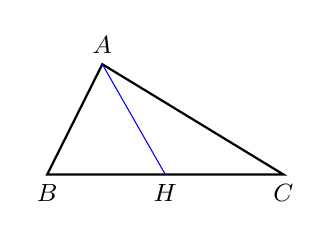
\begin{tikzpicture}[scale=1,font=\small]
\usetikzlibrary{calc}

\begin{scope}

\coordinate (b) at (0,0);
\coordinate (a) at (0.7,1.4);
\coordinate (c) at (3,0);

\draw[thick] (b) node[below] {$B$} -- (c) node[below] {$C$} -- (a) node[above] {$A$} -- cycle;

\coordinate (h) at ($(b)!0.5!(c)$);

\draw[blue] (h) node[black,below] {$H$} -- (a); % mediana
\end{scope}

\end{tikzpicture}

\end{minipage}
\end{esercizio}

% figura

\begin{esercizio}[Prove invalsi 2003]
\label{ese:2.100}
Da un triangolo equilatero $MNO$ di lato 6~cm viene tagliato via un triangolo equilatero di vertice in $O$ e lato 2~cm. Il perimetro del quadrilatero rimanente è \ldots
\begin{multicols}{5}
\begin{enumeratea}
\item 12~cm;
\item 14~cm;
\item 16~cm;
\item 18~cm;
\item 20~cm.
\end{enumeratea}
\end{multicols}
\end{esercizio}


\cleardoublepage
